
\chapter{幂级数与形式函数定理}
\label{ch:formal-functions}

幂级数是解析几何中的核心工具。它在代数几何中的类比——完备化——同样有用。我们只会触及这一主题的某些方面。
在 \S28.1 中，我们处理一些代数预备知识。\S28.2 中，我们用完备化（终于）给出一个定义……（我们在后续内容中会用到这些定义。）\S28.3 中，我们陈述本章的主要技术结果，即\mbox{形式函数定理~28.3.2}。随后的三节给出应用。\S28.4 中，我们证明\mbox{扎里斯基连通性引理~28.4.1} 与\mbox{斯坦因子分解定理~28.4.3}。\S28.5 中，我们证明（Grothendieck 版本的）扎里斯基主定理的一个常用版本，即\mbox{定理~28.5.1}；我们依赖 \S28.4。\S28.6 中，我们证明收缩 $(-1)$-曲线的 \trCastelnuovo{}判别准则，它在第 27 章中被我们用过。\trCastelnuovo{}判别准则的证明同样用到 \S28.4。最后，\S28.7 中我们证明\mbox{形式函数定理~28.3.2}。
本章刻意设置了大量小节，好让你看到它们大多并不像看上去那么难——例外是\mbox{形式函数定理~28.3.2} 本身的证明，以及将完备化与正合性、平坦性联系起来的\mbox{定理~28.1.6}。


\section{代数预备}

设 $A$ 是一个\trRing，而 $J_1\supset J_2\supset\cdots$ 是一个递减的\trIdeal{}序列。极限 $\lim A/J_n$ 常被记作 $\hat{A}$，并称为 $A$ 的\trCompletion（针对这一列\trIdeal）；这列\trIdeal{}则被隐去不言。\trCompletion{}最重要的情形是 $J_n=I^n$，其中 $I$ 是 $A$ 的一个\trIdeal。极限 $\lim A/I^n$ 称为\textbf{$A$ 的 $I$-进\trCompletion}（$I$-adic completion of $A$），或\textbf{$A$ 沿 $I$ 的\trCompletion}或\textbf{在 $I$ 处的\trCompletion}。

\textbf{28.1.1. \trhExample。}\quad 我们把 $k[[x_1,\dots,x_n]]$ 定义为 $k[x_1,\dots,x_n]$ 在\trMaximalIdeal{} $(x_1,\dots,x_n)$ 处的\trCompletion。这是 $k$ 上 $n$ 个变量的\trFormalPowerSeries{}环（\mbox{例~1.3.3}）。

\trPadics{}（\mbox{例~1.3.4}）是另一个例子。

\textbf{28.1.A.（练习）}\quad 设 $J'_1\supset J'_2\supset\cdots$ 是一个与 $J_n$ \textbf{共尾}（cofinal）的递减\trIdeal{}序列。换言之，对每个 $J_n$，存在某个 $J'_N$ 使得 $J_n\supset J'_N$；而对每个 $J'_n$，存在某个 $J_N$ 使得 $J'_n\supset J_N$。证明：存在\trCanonical{}\trIsomorphism
\[
\lim A/J'_n \xleftrightarrow{\ \sim\ } \lim A/J_n.
\]
于是，真正要紧的与其说是\trIdeal{}序列的具体样貌，不如说是其「共尾」\trEquivalenceClass。

\textbf{28.1.2. 预备注记。}\quad 我们有一个显然的\trMorphism{} $A\to\hat{A}$。

若在 $A/J_n$ 上赋予\trDiscreteTopology，则 $\hat{A}$ 自然而然地具有\textbf{拓扑环}（topological ring）的结构（所谓拓扑环，就是同时是一个\trTopologicalSpace{}的\trRing，其中一切环运算都是连续的；等价地说，即\trTopologicalSpace{}\trCategory{}中的一个\trRing{}对象）。于是我们还可以谈论拓扑环 $A'$ 上的\textbf{拓扑模}（topological module）$M$——即底\trRing{} $A'$ 上的一个\trModule，带有拓扑，使得 $A'$ 在 $M$ 上的作用是连续的。这是一种有用的观点，但我们不会用到它。

\textbf{28.1.B.（练习）}\quad 设 $\mathfrak{m}$ 是环 $A$ 的一个\trMaximalIdeal。证明：$A$ 在 $\mathfrak{m}$ 处的\trCompletion{}\trCanonical{}地\trIsomorphic{}于 $A_{\mathfrak{m}}$ 在 $\mathfrak{m}$ 处的\trCompletion。

若 $(A,\mathfrak{m})$ 是\trNoether{}\trLocalRing，则自然映射 $A\to\hat{A}$ 是\trInjectiveMap：\trKernel{}中的任何元素都必定落在 $\bigcap\mathfrak{m}^i$ 中，而由\trKrull{}交定理（\mbox{练习~13.9.A}(b)），后者为 $0$。于是「完备化不丢失任何信息」，正如（局部地看）解析函数由其幂级数展开所决定。

（在\trIdeal{} $I$ 处取\trCompletion{}的情形，若 $A\to\hat{A}$ 是\trInjectiveMap，则称 $A$ 是 \textbf{$I$-进分离}的（$I$-adically separated）；若 $A\to\hat{A}$ 是\trIsomorphism，则称 $A$ \textbf{对 $I$ 完备}（complete with respect to $I$）——尽管我们用不到这些措辞。例如，\trKrull{}交定理蕴含：若 $I$ 是\trNoether{}\trIntegralDomain{}或\trNoether{}\trLocalRing{}的一个\trProperIdeal，则 $A$ 是 $I$-进分离的。）

\textbf{28.1.C.（练习）}\quad 设 $(A,\mathfrak{m})$ 是一个包含其\trResidueField{} $k$ 的\trNoether{}\trLocalRing（也就是说，它是一个 $k$-\trAlgebra）。设 $x_1,\dots,x_n$ 是 $A$ 的若干元素，其在 $\mathfrak{m}/\mathfrak{m}^2$ 中的像构成一组基。证明：$k$-代数映射
\begin{equation*}
\tag{28.1.2.1}\label{eq:formal-series-to-completion}
k[[t_1,\dots,t_n]]\longrightarrow\hat{A}
\end{equation*}
（由 $t_i\mapsto x_i$ 定义）是满射。（请先解释为什么\emph{存在}这样的映射！）照例，对\trLocalRing{}而言，\trCompletion{}默认取在\trMaximalIdeal{}处。

\mbox{练习~28.1.C} 是\emph{\trCohen{}结构定理}（Cohen Structure Theorem）的特例。（关于这一话题的更多内容，见 [E, \S7.4]。）

\textbf{28.1.D.（练习）}\quad 设 $X$ 是 $k$ 上的一个\trLocally\trNoether{}\trScheme，而 $p\in X$ 是一个\trRationalPoint{}（$k$-\trValuedPoint）。设 $p\in X$ 是\trRegular{}的，\trCodimension{}为 $d$（即 $\dim\OO_{X,p}=d$）。请描述一个作为拓扑环的\trIsomorphism{} $\hat{\OO}_{X,p}\xleftrightarrow{\ \sim\ }k[[x_1,\dots,x_d]]$。（提示：如\mbox{练习~28.1.C} 中那样，选取 $\mathfrak{m}$ 的 $d$ 个元素，使其在 $\mathfrak{m}/\mathfrak{m}^2$ 中的像构成一组基；它们将是你的 $x_1,\dots,x_d$。证明：映射 \eqref{eq:formal-series-to-completion} 没有核。利用\mbox{定理~22.3.8} 把 $\mathfrak{m}^n/\mathfrak{m}^{n+1}$ 等同于 $\Sym^n(\mathfrak{m}/\mathfrak{m}^2)$ 或许有帮助。）

逆命题同样成立：若 $(A,\mathfrak{m},k)$ 是一个作为 $k$-代数的\trNoether{}\trLocalRing，且 $\hat{A}\cong k[[x_1,\dots,x_d]]$，则 $A$ 是一个 $d$ 维的\trRegular\trLocalRing；关键一步见 [AtM, Prop.~11.24]。

\textbf{28.1.3. \trhRemark。}\quad 设 $p$ 是 $d$ 维 $k$-\trVariety{}上的一个光滑的有理（$k$-值）点，并设 $f\in\OO_{X,p}$（$f$ 是一个「局部函数」）。借助\mbox{练习~28.1.D} 的\trIsomorphism，我们可以把 $f$ 解读为 $k[[x_1,\dots,x_d]]$ 中的一个元素。这应当被解读为「$f$ 在 $p$ 处的幂级数展开」，展开于「局部坐标 $x_1,\dots,x_d$」之下。

\textbf{28.1.4. 一些更多的几何动机。}\quad \mbox{练习~28.1.D} 或许能为\trCompletion{}给出一点动机：「在\trCompletion{}中，\trRegular\trScheme{}看起来像仿射空间」。这句话常以富有暗示性的语言陈述为「形式局部地，正则概形同构于仿射空间」；\S28.3.1 将把这一点说得略微更精确些。

我们现在再给出一点\trCompletion{}的几何动机，后面不会用到它。回想 \S13.6.1：平展\trMorphism{}被设计得看起来像微分几何中的「局部同构」。但\mbox{练习~13.6.F} 表明，这个比喻在一个重要方面败得很惨。更精确地说：令 $Y=\Spec k(t)$，$X=\Spec k[u,1/u]$，令 $p\in X$ 由 $u=1$ 给出，而 $q\in Y$ 由 $t=1$ 给出。设 $\operatorname{char}k\ne 2$。由 $t\mapsto u^2$ 诱导的\trMorphism{} $\pi\colon X\to Y$ 是平展的，且 $\pi(p)=q$。但 $p$ 不存在这样的开邻域，使得 $\pi$ 把它\trIsomorphic{}地映到 $q$ 的某个开邻域上。然而，下面的练习将表明：$\pi$ 诱导\trCompletion{}之间的\trIsomorphism（即「形式邻域」之间的\trIsomorphism）。

\textbf{28.1.E.（练习）}\quad 沿用上一段的记号，证明：$\pi$ 诱导\trCompletion{}之间的\trIsomorphism{} $\hat{\OO}_{Y,q}\to\hat{\OO}_{X,p}$。

\textbf{28.1.F.（练习）}\quad 设 $Y=\Spec A$，$X=\Spec A[t]/(f(t))$，而 $\pi\colon X\to Y$ 是由 $A\to A[t]/(f(t))$ 诱导的\trMorphism。设 $p\in X$ 是\trClosedPoint，$q\in Y$ 是\trClosedPoint，$\pi(p)=q$，且 $\pi$ 在 $p$ 处平展并诱导\trResidueField{}之间的\trIsomorphism。证明：$\pi$ 诱导\trCompletion{}之间的\trIsomorphism{} $\hat{\OO}_{Y,q}\to\hat{\OO}_{X,p}$。（如果你还不熟悉\textbf{\trHensel{}引理}（Hensel's Lemma），你或许会在解这道题的过程中重新发现它的核心思想。）

稍加细心，你便可以更一般地证明：若 $\pi\colon X\to Y$ 是平展\trMorphism，$\pi(p)=q$，且 $\pi$ 在 $p$ 处诱导\trResidueField{}之间的\trIsomorphism，则 $\pi$ 诱导\trCompletion{}之间的\trIsomorphism{} $\hat{\OO}_{Y,q}\to\hat{\OO}_{X,p}$。（你甚至可能想琢磨一下，如何去掉\trResidueField{}之间\trIsomorphism{}这一假设。）

这些想法与 \S24.8.13 中讨论的「形式\trEtale」定义相去不远。

你可以把这些结果解读为这样的陈述：「隐函数定理在形式局部上管用」，尽管它在扎里斯基局部上并不管用。（平展\trTopology{}介于这两者之间；它的部分设计意图，正是让这种意义下的隐函数定理总是成立——这纯粹是约定使然。但此处不宜讨论平展\trTopology。）

下面还有两个有趣的问题，它们暗地里讲的都是\trHensel{}引理。

\textbf{28.1.G.（练习）}\quad 证明：$x^2+y^2=-2$ 在模 $7^{100}$ 之下有解。

\textbf{28.1.H.（练习）}\quad 设 $\mathbb{A}^2_{\mathbb{Q}}$ 中有一条平面\trCurve{} $f(x,y)=0$，而 $(0,a)$ 是它的一个光滑点，其\trTangentLine{}非竖直。证明：恰好存在一个幂级数解 $y=p(x)$，使得 $f(x,p(x))=0$（作为幂级数），并且 $p(0)=a$。

\textbf{28.1.5. \trCompletion{}与\trExactness。}\quad 我们用一个有趣而有用的陈述来结束本节。

\textbf{28.1.6. \trhTheorem。}\ ——\ \emph{设 $A$ 是\trNoether{}环，而 $I\subset A$ 是一个\trIdeal。对任意 $A$-\trModule{} $M$，令 $\hat{M}=\lim M/I^jM$ 为 $M$ 关于 $I$ 的\trCompletion。}

\emph{(a) \trCompletion{} $\hat{A}$（$A$ 关于 $I$ 的\trCompletion）在 $A$ 上\trFlat。}

\emph{(b) 若 $M$ 是有限生成的，则自然映射 $\hat{A}\otimes_A M\to\hat{M}$ 是\trIsomorphism。}

\emph{(c) 若 $0\to M\to N\to P\to 0$ 是有限生成 $A$-\trModule{}的一个\trShortExactSequence，则 $0\to\hat{M}\to\hat{N}\to\hat{P}\to 0$ 正合。（于是，由\mbox{练习~1.5.F}，\trCompletion{}保持有限生成\trModule{}的\trExactSequence。）}

我们将在 \S28.2 中用到 (a)，在 \S28.7 中用到 (b)。

\textbf{28.1.7. \trhRemark。}\quad 在证明\mbox{定理~28.1.6} 之前，我们先作一些注记。(a) 与 (b) 合在一起显然蕴含 (c)，但我们却要用 (c) 来证明 (a) 与 (b)。另外，注意一个微妙的区别（它帮助我记住这个陈述）：若 $0\to M\to N\to P\to 0$ 是 $A$-\trModule{}的一个\trExactSequence，其中的模\emph{未必有限生成}，则
\begin{equation*}
\tag{28.1.7.1}\label{eq:completion-tensor-exact}
0\longrightarrow \hat{A}\otimes_A M\longrightarrow \hat{A}\otimes_A N\longrightarrow \hat{A}\otimes_A P\longrightarrow 0
\end{equation*}
\emph{总是}正合，但
\begin{equation*}
\tag{28.1.7.2}\label{eq:completion-itself-exact}
0\longrightarrow \hat{M}\longrightarrow \hat{N}\longrightarrow \hat{P}\longrightarrow 0
\end{equation*}
\emph{未必}正合——而当它\emph{的确}正合时，往往是因为这些\trModule{}是有限生成的，从而 \eqref{eq:completion-itself-exact} 其实就是 \eqref{eq:completion-tensor-exact}。

当心：\trCompletion{}并不总是正合的。考虑 $k[t]$-\trModule{}的正合列
\[
0\longrightarrow \bigoplus_{n=1}^{\infty}k[t]\xrightarrow{\ \times(t,t^2,t^3,\dots)\ }\bigoplus_{n=1}^{\infty}k[t]\longrightarrow \bigoplus_{n=1}^{\infty}k[t]/(t^n)\longrightarrow 0.
\]
对理想 $((t,t,t,\dots))$ 作\trCompletion{}之后，这个序列在中间不再正合：$(t^2,t^3,t^4,\dots)$ 被映到 $0$，但它并不在前一项的\trCompletion{}的像中。

\extrahard\ \emph{证明。}\quad 关键的一步是证明 (c)，我们通过一连串练习来完成它。设 $0\to M\to N\to P\to 0$ 是有限生成 $A$-\trModule{}的一个\trShortExactSequence。

\textbf{28.1.I.（练习）}\quad 证明：$\hat{N}\to\hat{P}$ 是满射。提示：把 $\hat{P}$ 的一个元素看成序列 $(p_j\in P/I^jP)_{j\ge 0}$，其中 $p_{j+1}$ 的像是 $p_j$；参看\mbox{练习~1.3.C}。对 $j$ 作归纳，构造出原像 $(n_j\in N/I^jN)_{j\ge 0}$。

我们现在希望把 $\ker(\hat{N}\to\hat{P})$ 等同于 $\hat{M}$。

\textbf{28.1.J.（练习）}\quad 证明：对每个 $j\ge 0$，
\begin{equation*}
\tag{28.1.7.3}\label{eq:ses-mod-intersection}
0\longrightarrow M/(M\cap I^jN)\longrightarrow N/I^jN\longrightarrow P/I^jP\longrightarrow 0
\end{equation*}
是正合的。（一个可能的提示：证明 $0\to M\cap I^jN\to M\to N/I^jN\to P/I^jP\to 0$ 正合。）

这些短正合列 \eqref{eq:ses-mod-intersection} 随着 $j$ 的变动构成一个\trInverseSystem。它的极限是\trLeftExact{}的（极限总是如此），但由\mbox{练习~1.5.N}，它还是\trRightExact{}的，因为「左边的\trTransitionMap{}」$M/(M\cap I^{j+1}N)\to M/(M\cap I^jN)$ 显然是满射。于是
\begin{equation*}
\tag{28.1.7.4}\label{eq:limit-ses}
0\longrightarrow \lim M/(M\cap I^jN)\longrightarrow \hat{N}\longrightarrow \hat{P}\longrightarrow 0
\end{equation*}
正合。为了完成 (c) 的证明，只需（由\mbox{练习~28.1.A}）证明：子模序列 $I^jM$ 与序列 $M\cap I^jN$ 共尾，从而 \eqref{eq:limit-ses} 左端的项 $\lim M/(M\cap I^jN)$ 便自然而然地等同于 $\hat{M}$。

\textbf{28.1.K.（练习）}\quad 证明这一点。提示：显然，$I^jM\subset M\cap I^jN$。由\trArtin--\trRees{}引理~13.9.3 的\trCorollary{}~13.9.4，对某个整数 $s$，对一切 $j\ge 0$ 都有 $M\cap I^{j+s}N=I^j(M\cap I^sN)$，而显然 $I^j(M\cap I^sN)\subset I^jM$。

这就完成了\mbox{定理~28.1.6} 的部分 (c) 的证明。

对于部分 (b)，把 $M$ 呈现为
\begin{equation*}
\tag{28.1.7.5}\label{eq:presentation-of-m}
A^{\oplus m}\xrightarrow{\ \alpha\ }A^{\oplus n}\longrightarrow M\longrightarrow 0,
\end{equation*}
其中 $\alpha$ 是一个系数取在 $A$ 中的 $m\times n$ 矩阵。在这一情形下，由部分 (c)，\trCompletion{}是正合的，而且它显然与有限\trDirectSum{}交换，于是
\[
\hat{A}^{\oplus m}\longrightarrow \hat{A}^{\oplus n}\longrightarrow \hat{M}\longrightarrow 0
\]
是正合的。\trTensorProduct{}是\trRightExact{}的，并且与\trDirectSum{}交换（\mbox{练习~1.2.M}），于是
\[
\hat{A}^{\oplus m}\longrightarrow \hat{A}^{\oplus n}\longrightarrow \hat{A}\otimes_A M\longrightarrow 0
\]
也是正合的。注意，这两列\trRightExact{}的序列中从 $\hat{A}^{\oplus m}$ 到 $\hat{A}^{\oplus n}$ 的映射是相同的；它们都是 $\alpha$。于是二者的\trCokernel{}得到等同，(b) 随之得证。

最后，为了证明 (a)，我们需要把平坦性的理想论判别法（\mbox{定理~24.3.1}）稍作推广。回想（\S24.3.2）：它等价于下述事实——$A$-\trModule{} $M$ 是\trFlat{}的，当且仅当对一切\trIdeal{} $I$，自然映射 $I\otimes_A M\to M$ 都是\trInjectiveMap。

\textbf{28.1.L.（练习：平坦性的理想论判别法的加强形式）}\quad 证明：$A$-\trModule{} $M$ 是\trFlat{}的，当且仅当对一切\emph{有限生成}的\trIdeal{} $I$，自然映射 $I\otimes_A M\to M$ 都是\trInjectiveMap。（提示：若对某个非有限生成的\trIdeal{} $J$ 有反例，就用它找出另一个对\emph{确为}有限生成的\trIdeal{} $I$ 的反例。）

依这条判别法，为证 (a)，只需证明：对一切有限生成的\trIdeal{} $I$，乘法映射 $I\otimes_A\hat{A}\to\hat{A}$ 都是\trInjectiveMap。但由部分 (b)，这与证明 $\hat{I}\to\hat{A}$ 是\trInjectiveMap 是同一回事\footnote{译注：原书此处作「this is the same showing that」，当为「this is the same as showing that」之误（脱漏 as），径改。——译者注}；而这由部分 (c) 即得。\hfill$\square$


\section{奇点的类型}

奇点往往用\trCompletion{}来定义最为简捷。

\textbf{28.2.1. \trhDefinition。}\quad 设 $X$ 是 $\bar{k}$ 上维数为 $1$ 的\trVariety，而 $p\in X$ 是一个\trClosedPoint。若 $\OO_{X,p}$ 在 $\mathfrak{m}_{X,p}$ 处的\trCompletion{}（作为拓扑环）\trIsomorphic{}于 $\bar{k}[[x,y]]/(xy)$，则称 $X$ 在 $p$ 处有一个\textbf{\trNode}。（这与 \S13.3.2 中\trNode{}的定义相比如何？）

\textbf{28.2.A.（练习）}\quad 设 $k=\bar{k}$ 且 $\operatorname{char}k\neq 2$。证明：$\mathbb{A}^2_k$ 中由 $y^2=x^2+x^3$ 截出的\trCurve{}在原点处有一个\trNode{}——自\cref{fig:normalization-nodal-cubic} 起，我们已经反复研究过这条曲线了。

\textbf{28.2.B.（练习）}\quad 设 $k=\bar{k}$，$\operatorname{char}k\neq 2$，并设有 $f(x,y)\in k[x,y]$。

(a)~证明：$\Spec k[x,y]/(f(x,y))$ 在原点处有一个\trNode，当且仅当 $f$ 没有次数为 $0$ 或 $1$ 的项，且其次数为 $2$ 的项不是一个完全平方。（这推广了\mbox{练习~28.2.A}。）

(b)~证明：$\Spec k[x,y]/(f(x,y))$ 在点 $(a,b)$ 处有一个\trNode，当且仅当
\[
\frac{\partial f}{\partial x}=\frac{\partial f}{\partial y}=0
\qquad\text{且}\qquad
\left(\frac{\partial^2 f}{\partial x^2}\right)\left(\frac{\partial^2 f}{\partial y^2}\right)\neq\left(\frac{\partial^2 f}{\partial x\,\partial y}\right)^{\!2}
\]
在 $(a,b)$ 处成立。

对于代数闭域上的\trVariety{}之外的情形，\trNode{}的定义要更成问题，我们给出几条可能的进路。对非代数闭域 $k$ 上的\trVariety，总可以\trBaseChange{}到代数闭包 $\bar{k}$。作为另一条进路，若 $p$ 是 $k$ 上（未必代数闭的）\trVariety{}的一个 $k$-\trValuedPoint，那么也可以径取同一个\mbox{定义~28.2.1}；如此得到的奇点可以合理地称作\emph{\trSplitNode}（split node），因为诸分支（或者更确切地说，诸切方向）是可分辨的。那些并\trNonSplitNode、但在\trBaseChange{}到 $\bar{k}$ 之后成为\trNode{}的奇点——诸如 $\Spec\mathbb{R}[x,y]/(x^2+y^2)$ 或 $\Spec\mathbb{Q}[x,y]/(x^2-2y^2)$ 的原点——可以合理地称作\emph{\trNonSplitNode}（non-split node）。

\textbf{28.2.2. \trhDefinition。}\quad 我们可以用类似的方式定义其他奇点。为免生枝节，我们在代数闭域上作定义。设 $X$ 是 $\bar{k}$ 上的\trVariety，$p$ 是 $X$ 的一个\trClosedPoint，其中 $\operatorname{char}k\neq 2$、$3$。若 $\hat{\OO}_{X,p}$ \trIsomorphic{}于 $\bar{k}[x,y]/(y^2-x^3)$ 的\trCompletion（相应地，$\bar{k}[x,y]/(y^2-x^4)$、$\bar{k}[x,y]/(y^3-x^3)$ 的\trCompletion），则称 $X$ 在 $p$ 处有一个\textbf{\trCusp}（相应地，\textbf{\trTacnode}、\textbf{\trTriplePoint{}}（triple point））。（前两种的图像见\cref{fig:plane-curve-singularities}。）若 $\hat{\OO}_{X,p}$ \trIsomorphic{}于 $\bar{k}[x,y]/(f(x,y))$ 的\trCompletion，其中 $f$ 是一个无重根的 $m$ 次\trHomogeneous{}多项式，则称 $X$ 在 $p$ 处有一个\textbf{重数 $m$ 的普通多重点}（ordinary multiple point of multiplicity $m$），或称\textbf{普通 $m$ 重点}（ordinary $m$-fold point）。（你可以很快看到：普通 $2$ 重点——或称\emph{普通二重点}（ordinary double point）——恰是一个\trNode，而普通 $3$ 重点是一个\trTriplePoint{}。）

\textbf{28.2.C.（平凡练习）}\quad （为简单起见，本练习在代数闭域上做。）定义 $A_n$ \textbf{曲线奇点}（curve singularity）（见 \S22.4.4）。定义 $A_n$ \textbf{曲面奇点}（surface singularity）（见\mbox{练习~22.4.F}）。定义 \textbf{$D_n$、$E_6$、$E_7$ 与 $E_8$ 曲面与曲线奇点}（surface and curve singularities）（见\mbox{注记~22.4.5}）。

\textbf{28.2.3. 使用这个定义。}\quad 现在我们给出一个例子，说明这个定义可以如何使用。

\textbf{28.2.D.（练习）}\quad 设 $X$ 是一个 $\bar{k}$-\trVariety，在\trClosedPoint{} $p$ 处有一个\trNode。证明：$X$ 在 $p$ 处的\trBlowup{}给出一个\trMorphism{} $\beta\colon\tilde{X}\to X$，其中\trExceptionalDivisor{} $\beta^{-1}(p)$ 由两个既约的光滑点组成。提示：利用「\trCompletion{}是\trFlat{}的」（\mbox{定理~28.1.6}(a)）与「胀开与平坦\trBaseChange{}交换」（\mbox{练习~24.1.P}(a)）这两个事实，把问题化归为对\trNode{}的「形式模型」$\Spec\bar{k}[x,y]/(xy)$ 的一个计算。

\textbf{28.2.E.（练习）}\quad 沿用上一个练习的术语，描述一个\trExactSequence
\begin{equation*}
\tag{28.2.3.1}\label{eq:node-blowup-ses}
0\longrightarrow\OO_X\longrightarrow\beta_*\OO_{\tilde{X}}\longrightarrow\OO_p\longrightarrow 0.
\end{equation*}
提示：\trFaithfullyFlat{}性。

\textbf{28.2.F.（练习）}\quad 我们沿用上两个练习的术语。设 $X$ 是纯维既约射影\trCurve，证明：$p_a(X)=p_a(\tilde{X})+1$。

于是，「解消一个\trNode」使\trCurve{}的\trArithmeticGenus{}减少 $1$。如果你愿意，你不难进一步证明：「解消一个\trCusp」使亏格减少 $1$，而「解消一个\trTacnode」使亏格减少 $2$。一般地，对每一类\trCurve\trSingularPoint，它对亏格的贡献——也就是（当\trCurve{}是射影时）这条\trCurve{}的亏格与其「在该\trSingularPoint{}处的部分\trNormalization」的亏格之差——称为\textbf{\trDeltaInvariant}（$\delta$-invariant）。于是，\trNode{}或\trCusp{}的 $\delta$ 为 $1$，而\trTacnode{}的 $\delta$ 为 $2$。

\textbf{28.2.G.（练习）}\quad 证明：对\emph{任何}奇点类型（除光滑点以外），都有 $\delta>0$。

\textbf{28.2.H.（练习）}\quad 证明：既约不可约的 $d$ 次平面\trCurve{}至多能有 $\binom{d-1}{2}$ 个\trSingularPoint。

\textbf{28.2.I.（练习）}\quad 有一个非正式的小窍门，可以在结点（射影既约）\trCurve{}于例子中出现时迅速算出其亏格。在画得出来的前提下，在一张纸上（也就是实平面）画一幅草图，使\trNode{}「看上去像\trNode」，并且亏格为 $g$ 的\trCurve{}被画有 $g$ 个洞，如\cref{fig:genus-count-sketch} 那样。（在\cref{fig:genus-count-sketch} 中，我们看到四个\trIrreducibleComponent，其\trGeometricGenus{}分别为 $0$、$0$、$1$ 与 $3$；前三个分量是光滑的，而第四个与自身相交一次；此外还有六个\trNode。）然后，若这条\trCurve{}\trConnected，就数一数图中看得见的洞的个数。证明这套口诀确实有效。（若\trCurve{}不连通时该怎么办，也请自行琢磨。）

\begin{figure}[htbp]
\centering
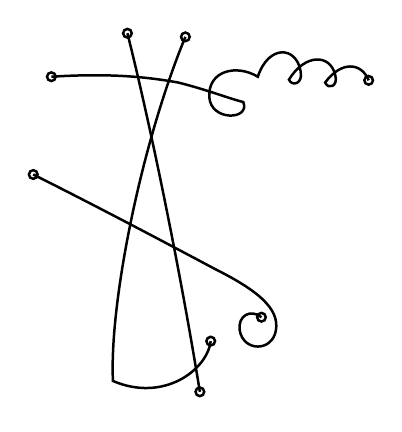
\begin{tikzpicture}[line width=0.9pt, scale=0.92]
  \draw (2.15,2.45) .. controls (1.55,1.00) and (1.10,-1.20) .. (1.15,-2.30)
        .. controls (1.85,-2.60) and (2.45,-2.15) .. (2.50,-1.75);
  \draw (1.35,2.50) .. controls (1.70,1.10) and (2.10,-0.90) .. (2.35,-2.45);
  \draw (0.05,0.55) .. controls (0.85,0.15) and (1.80,-0.35) .. (2.55,-0.75)
        .. controls (3.15,-1.05) and (3.45,-1.30) .. (3.40,-1.60)
        .. controls (3.35,-1.90) and (2.95,-1.90) .. (2.90,-1.60)
        .. controls (2.87,-1.40) and (3.05,-1.30) .. (3.20,-1.42);
  \draw (0.30,1.90) .. controls (1.10,1.95) and (1.60,1.90) .. (2.05,1.82)
        .. controls (2.45,1.72) and (2.75,1.60) .. (2.95,1.55)
        .. controls (3.05,1.30) and (2.50,1.28) .. (2.48,1.62)
        .. controls (2.46,1.98) and (2.85,2.08) .. (3.15,1.90)
        .. controls (3.30,2.35) and (3.68,2.32) .. (3.74,1.98)
        .. controls (3.78,1.80) and (3.62,1.76) .. (3.58,1.86)
        .. controls (3.80,2.22) and (4.15,2.22) .. (4.22,1.92)
        .. controls (4.26,1.76) and (4.12,1.72) .. (4.08,1.82)
        .. controls (4.30,2.12) and (4.58,2.10) .. (4.68,1.85);
  \draw (2.15,2.45) circle (1.7pt);
  \draw (2.50,-1.75) circle (1.7pt);
  \draw (1.35,2.50) circle (1.7pt);
  \draw (2.35,-2.45) circle (1.7pt);
  \draw (0.05,0.55) circle (1.7pt);
  \draw (3.20,-1.42) circle (1.7pt);
  \draw (0.30,1.90) circle (1.7pt);
  \draw (4.68,1.85) circle (1.7pt);
\end{tikzpicture}
\caption{这条\trCurve{}的亏格为 $8$（数一数那些「洞」！）。（依原书手绘图重绘。）}\label{fig:genus-count-sketch}
\end{figure}

\textbf{28.2.4.}\quad 这可能相当有用。例如，\cref{fig:arith-genus-sketches} 中的几幅草图可以提醒你：$d$ 次平面\trCurve{}的\trArithmeticGenus{}为 $\binom{d-1}{2}$；$\mathbb{P}^1\times\mathbb{P}^1$ 上由 $\OO(a,b)$ 的一个\trSection{}给出的\trCurve{}具有亏格 $(a-1)(b-1)$（\S15.2.10）；而 \trHirzebruchSurface{} $\mathbb{F}_2$ 上类为 $2C+2F$ 的\trCurve{}（使用\mbox{练习~20.2.M} 的语言）的\trArithmeticGenus{}为 $3$。在每一种情形，我们都是在该类中取一条合适的\trCurve，利用「\trArithmeticGenus{}在\trFlat\trFamily{}中是常数」这一事实（\mbox{关键练习~24.7.A}）。

\begin{figure}[htbp]
\centering
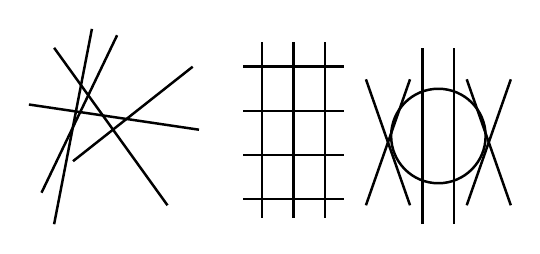
\begin{tikzpicture}[line width=0.9pt, scale=0.8]
  \draw (-0.10,2.40) -- (1.70,-0.10);
  \draw (0.90,2.60) -- (-0.30,0.10);
  \draw (-0.50,1.50) -- (2.20,1.10);
  \draw (0.20,0.60) -- (2.10,2.10);
  \draw (0.50,2.70) -- (-0.10,-0.40);
  \draw (3.20,-0.30) -- (3.20,2.50);
  \draw (3.70,-0.30) -- (3.70,2.50);
  \draw (4.20,-0.30) -- (4.20,2.50);
  \draw (2.90,0.00) -- (4.50,0.00);
  \draw (2.90,0.70) -- (4.50,0.70);
  \draw (2.90,1.40) -- (4.50,1.40);
  \draw (2.90,2.10) -- (4.50,2.10);
  \draw (6.00,1.00) circle (0.75);
  \draw (5.75,-0.40) -- (5.75,2.40);
  \draw (6.25,-0.40) -- (6.25,2.40);
  \draw (4.85,1.90) -- (5.55,-0.10);
  \draw (4.85,-0.10) -- (5.55,1.90);
  \draw (6.45,1.90) -- (7.15,-0.10);
  \draw (6.45,-0.10) -- (7.15,1.90);
\end{tikzpicture}
\caption{这三条\trCurve{}的\trArithmeticGenus{}分别为 $6$、$6$ 与 $3$。（依原书手绘图重绘。）}\label{fig:arith-genus-sketches}
\end{figure}

\textbf{28.2.5. 其他定义。}\quad 若 $\bar{k}=\mathbb{C}$，则这一类定义与解析定义相吻合（见 [Ar1, \S1]）。例如，一个复代数\trCurve\trSingularPoint{}是\trNode，当且仅当它\trAnalyticallyIsomorphic{}于 $\mathbb{C}^2$ 中 $xy=0$ 的一个开邻域。还有一种「平展局部」的\trIsomorphism{}概念，我们在此不作定义。同样地，这也导致这几类奇点的同一个定义（见 [Ar2, \S2]）。


\section{形式函数定理}

设 $\pi\colon X\to Y$ 是\trLocally\trNoether{}\trScheme{}之间的一个\trProper\trMorphism\footnote{原书此处作「is proper morphism」，当为「is a proper morphism」之误（脱漏冠词 a），径改。——译者注}，而 $\mathscr{F}$ 是 $X$ 上的一个\trCoherentSheaf，从而 $\mathrm{R}^1\pi_*\mathscr{F}$ 是一个\trCoherentSheaf（\mbox{\trGrothendieck{}凝聚定理~18.9.1}）。取定一点 $q\in Y$。我们已经有这样一种感觉：$\mathrm{R}^1\pi_*\mathscr{F}$ 在 $q$ 处的\trFiber{}与 $\mathscr{F}$「在纤维 $X_q$ 上」的\trCohomology{}之间的关系并不完美，而第 25 章的大量篇幅正是致力于把这一点说精确。

形式函数定理以另一种方式处理这个问题：它并不去比较 $\mathrm{R}^1\pi_*\mathscr{F}$ 的\trFiber{}与 $\mathscr{F}$ 限制到纤维上的\trCohomology，而是在关于纤维之「无穷小\trThickening{}」的信息之间给出一个\trIsomorphism。非正式地说：

\begin{center}
\begin{tikzpicture}[x=1cm,y=1cm,>=stealth,line width=0.5pt]
\node (A)  at (0,0)       {$\mathrm{R}^i\pi_*\mathscr{F}$};
\node (B0) at (7.4,0)     {$\mathrm{H}^i(X_q,\mathscr{F}|_{X_q})$};
\node (B1) at (7.4,-1.1)  {$\mathrm{H}^i(\text{$X_q$ 的 $0$ 阶邻域},\mathscr{F})$};
\node (B2) at (7.4,-2.2)  {$\mathrm{H}^i(\text{$X_q$ 的 $1$ 阶邻域},\mathscr{F})$};
\node (B3) at (7.4,-3.3)  {$\mathrm{H}^i(\text{$X_q$ 的 $2$ 阶邻域},\mathscr{F})$};
\node (V)  at (7.4,-4.2)  {$\vdots$};
\node (L)  at (7.4,-5.2)  {极限。};
\node (C)  at (0,-5.2)    {$\mathrm{R}^i\pi_*\mathscr{F}$ 在 $q$ 处的\trCompletion};
\draw[->] (A) -- (B0);
\draw[->] (A) -- (B1);
\draw[->] (A) -- (B2);
\draw[->] (A) -- (B3);
\draw[->] (A) -- (L);
\draw[->] (A) -- (C);
\draw[->] (C) -- (L) node[above,midway] {\scriptsize 定理~28.3.2：同构};
\draw[->] (L) -- (V);
\draw[->] (V) -- (B3);
\draw[->] (B3) -- (B2);
\draw[->] (B2) -- (B1);
\draw[double,double distance=1.2pt] (B1) -- (B0);
\end{tikzpicture}
\end{center}

\textbf{28.3.1.}\quad 现在我们把这一点说得更加精确。若 $Z$ 是 $W$ 中由\trIdealSheaf{} $\mathscr{I}$ 截出的一个\trClosedSubscheme，我们就称由 $\mathscr{I}^{n+1}$ 截出的那个\trClosedSubscheme{}为 $Z$（在 $W$ 中）的\textbf{$n$ 阶形式}（或\textbf{无穷小}）\textbf{邻域}（或\textbf{\trThickening{}}）（nth order formal (or infinitesimal) neighborhood (or thickening)）。不提「阶」而单说「形式邻域」时，指的是同时蕴于所有这些邻域之中的信息，其形态往往是我们马上就要描述的那种极限。（这也会把我们引向\trFormalScheme{}的概念——尽管很重要，我们却终究用不到。）

现在转向我们感兴趣的情境。我们不看 $\mathrm{R}^i\pi_*\mathscr{F}$ 在 $q$ 处的\trFiber，而看它的\trCompletion：取其在 $q$ 处的\trStalk，然后在\trMaximalIdeal{} $\mathfrak{m}_q$ 处作\trCompletion。我们不看 $\mathscr{F}$ 沿纤维的\trCohomology，而看 $\mathscr{F}$ 限制到纤维的 $n$ 阶形式邻域 $X_n$ 上时的\trCohomology，并取极限。形式函数定理说，这两者被\trCanonically{}等同。

在陈述形式函数定理之前，我们需要把这些极限究竟是什么、又如何定义说清楚。为了专注于本质，我们在 $q$ 是 $Y$ 的一个\emph{\trClosedPoint}的特殊情形下做这件事，而把（温和的）到一般情形的推广留给你（\mbox{练习~28.3.A}）。

我们先来处理 $\mathrm{R}^i\pi_*\mathscr{F}$。注意到下面这点很有帮助：由\mbox{练习~28.1.B}，要计算限制到第 $n$ 个形式邻域上的结果，既可以通过拉回到 $\Spec\OO_{Y,q}$（即「$Y$ 在 $q$ 处的\trGerm」，也就是与 $\OO_{Y,q}$ 作张量）来实现，也可以在 $q\in Y$ 的任何一个仿射开邻域中实现。为方便起见，我们选取 $q$ 的一个仿射开邻域 $\Spec B\subset Y$。（同样由\mbox{练习~28.1.B}，选取哪个仿射开子集并不要紧。）为方便起见，令 $X_B:=\pi^{-1}(\Spec B)$。设 $\mathfrak{m}\subset B$ 是对应于 $q$ 的\trMaximalIdeal。于是 $\widehat{(\mathrm{R}^i\pi_*\mathscr{F})_q}$ \trCanonically{}就是\trCoh{} $B$-模 $\mathrm{H}^i(X_B,\mathscr{F}|_{X_B})$ 在 $\mathfrak{m}$ 处的\trCompletion：
\[
\widehat{(\mathrm{R}^i\pi_*\mathscr{F})_q}
=\lim\ \mathrm{H}^i(X_B,\mathscr{F}|_{X_B})/\mathfrak{m}^n\mathrm{H}^i(X_B,\mathscr{F}|_{X_B}).
\]

接下来看 $\mathscr{F}$ 在纤维的\trThickening{}上的\trCohomology。我们有闭嵌入 $X_n\hookrightarrow X_{n+1}$，从而有\trCohomology{}群之间的映射
\[
\mathrm{H}^i(X_{n+1},\mathscr{F}|_{X_{n+1}})
\longrightarrow
\mathrm{H}^i(X_n,\mathscr{F}|_{X_n}).
\]
我们有基变换映射
\begin{equation*}
\tag{28.3.1.1}\label{eq:base-change-map-finite-level}
\mathrm{H}^i(X_B,\mathscr{F}|_{X_B})/\mathfrak{m}^n\mathrm{H}^i(X_B,\mathscr{F}|_{X_B})
\longrightarrow
\mathrm{H}^i(X_n,\mathscr{F}|_{X_n})
\end{equation*}
（见 \eqref{eq:natural-pushpull-morphism}），使得方块
\[
\begin{tikzcd}[row sep=2.8em, column sep=4em]
\mathrm{H}^i(X_B,\mathscr{F}|_{X_B})/\mathfrak{m}^{n+1}\mathrm{H}^i(X_B,\mathscr{F}|_{X_B})
\ar[r]\ar[d] &
\mathrm{H}^i(X_{n+1},\mathscr{F}|_{X_{n+1}})
\ar[d] \\
\mathrm{H}^i(X_B,\mathscr{F}|_{X_B})/\mathfrak{m}^n\mathrm{H}^i(X_B,\mathscr{F}|_{X_B})
\ar[r] &
\mathrm{H}^i(X_n,\mathscr{F}|_{X_n})
\end{tikzcd}
\]
交换。（你明白为什么吗？基本上，这同样是因为它们是基变换映射。）于是我们有一个诱导的极限之间的映射：
\begin{equation*}
\tag{28.3.1.2}\label{eq:limit-map}
\widehat{(\mathrm{R}^i\pi_*\mathscr{F})_q}
\longrightarrow
\lim_{n\to\infty}\mathrm{H}^i(X_n,\mathscr{F}|_{X_n}).
\end{equation*}

\textbf{28.3.A.（练习）}\quad 把前面的讨论推广到 $q$ 不是 $Y$ 的\trClosedPoint{}的情形。

形式函数定理断言，这是一个\trIsomorphism。

\textbf{28.3.2. 形式函数定理。}\ ——\ \emph{设 $\pi\colon X\to Y$ 是\trLocally\trNoether{}\trScheme{}之间的一个\trProper\trMorphism，$\mathscr{F}$ 是 $X$ 上的一个\trCoherentSheaf，而 $q\in Y$。则对一切 $i\ge 0$，\eqref{eq:limit-map} 都是\trIsomorphism。}

\trhWarning{}：形式函数定理并\emph{不}蕴含任何关于「有限层」上的映射的断言，即关于「有限 $n$」的 \eqref{eq:base-change-map-finite-level} 的断言。

\mbox{定理~28.3.2} 的证明颇为微妙，被推迟到带双星（\extrahard）的 \S28.7。为了让你保持动力、跃跃欲试，我们先给出如下四个重要应用：\mbox{\trZariski{}连通性引理~28.4.1}、\mbox{\trStein{}因子分解定理~28.4.3}、\mbox{\trZariskiMainTheorem~28.5.1}，以及关于收缩曲面上 $(-1)$-曲线的\mbox{\trCastelnuovo{}判别准则~28.6.1}。




\section{\trZariski{}连通性引理与\trStein{}因子分解}

我们现在来陈述并证明\trZariski{}连通性引理，它曾在 \S25.1.8 中被提及。

\textbf{28.4.1. \trZariski{}连通性引理。}\ ——\ \emph{若局部\trNoether{}\trScheme{}之间的一个\trProper\trMorphism{} $\pi\colon X\to Y$ 是 $\OO$-连通的（见 \S25.1.7），则对每个 $q\in Y$，$\pi^{-1}(q)$ 都是\trConnected{}的。}

该证明需要下面的结果。

\textbf{28.4.A.（容易练习：局部环的完备化是局部环）}\quad 设 $(A,\mathfrak{m})$ 是一个\trNoetherian\trLocalRing。证明：$A$ 沿 $\mathfrak{m}$ 的\trCompletion，即 $\hat{A}:=\lim A/\mathfrak{m}^n$，是一个\trLocalRing，其\trMaximalIdeal{}为 $\mathfrak{m}\hat{A}$。提示：证明 $\hat{A}$ 中任何不属于 $\mathfrak{m}\hat{A}$ 的元素都\trInvertible。

\emph{证明。}\quad 假设不然：存在某个 $q\in Y$ 使得 $\pi^{-1}(q)$ 不\trConnected，比方说 $\pi^{-1}(q)=X_1\coprod X_2$（其中 $X_1$ 与 $X_2$ 是这条\trFiber{}的两个非空\trOpenSubset；见\cref{fig:formal-neighborhoods}）。于是 $\pi^{-1}(q)$ 的 $n$ 阶形式邻域，由于带有同一个\trTopologicalSpace，也是不\trConnected{}的。我们使用\trIdempotent{}这一实用技巧（\mbox{注记~3.6.3}）。令 $e_1$ 为在 $X_1$ 上取值 $1$、在 $X_2$ 上取值 $0$ 的函数，并令 $e_2$ 为在 $X_2$ 上取值 $1$、在 $X_1$ 上取值 $0$ 的函数。这些函数在任何阶的形式邻域上都有意义，而且它们在\trInverseLimit{}中有自然的像。由\mbox{形式函数定理~28.3.2} 给出的\trIsomorphism（施用于 $\mathrm{H}^0$），我们得到 $\hat{\OO}_{Y,q}$ 中的非零元 $e_1$ 与 $e_2$，满足 $e_1+e_2=1$、$e_1e_2=0$。此时，$\hat{\OO}_{Y,q}$ 是一个\trLocalRing（\mbox{练习~28.4.A}）。但 $e_1e_2=0$ 蕴含 $e_1$ 与 $e_2$ 都不\trInvertible（否则另一个就会是 $0$），于是 $e_1$ 与 $e_2$ 都落在\trMaximalIdeal{}中，从而 $e_1+e_2$ 不可能是 $1$。我们由此得到矛盾。\hfill$\square$

\begin{figure}[htbp]
\centering
\begin{tikzpicture}[x=1cm,y=1cm,>=stealth,line width=0.5pt]
\node (X1) at (1.45,0.75)  {$X_1$};
\node (X2) at (1.55,0.05)  {$X_2$};
\draw[->,densely dashed] (0.55,0.75) -- (1.05,0.75);
\draw[->,densely dashed] (0.65,0.05) -- (1.15,0.05);
\draw[->,gray!70!black!60,line width=0.9pt] (0.95,-0.5) -- (0.95,-2.25);
\node at (0.95,-2.62) {$\bullet$};
\node at (0.95,-3.0)  {$q$};
\draw[line width=0.6pt] (-1.3,-2.55) .. controls (-0.5,-2.8) and (0.1,-2.45) ..
      (0.95,-2.62) .. controls (1.8,-2.8) and (2.4,-2.5) .. (2.75,-2.4);
\node at (3.15,-2.2) {$Y$};
\end{tikzpicture}
\caption{\mbox{\trZariski{}连通性引理~28.4.1} 证明中 $X_1$ 与 $X_2$ 的「形式邻域」。（依原书手绘图重绘。）}
\label{fig:formal-neighborhoods}
\end{figure}

\textbf{28.4.2. \trStein{}因子分解。}\quad 我们接下来描述那个被称为「\trStein{}因子分解」（Stein factorization）的构造。我们本可以早早地就把它定义出来，但现在，\mbox{\trZariski{}连通性引理~28.4.1} 将给我们带来一些令人瞩目的推论。

\textbf{28.4.3. \trStein{}因子分解定理。}\ ——\ \emph{任何局部\trNoether{}\trScheme{}之间的\trProper\trMorphism{} $\pi\colon X\to Y$ 都可以分解为 $\beta\circ\alpha$，其中 $\alpha\colon X\to Y'$ 是\trProper{}且 $\OO$-连通的（从而由\mbox{\trZariski{}连通性引理~28.4.1}，它具有\trConnected{}的\trFiber），而 $\beta\colon Y'\to Y$ 是一个\trFinite\trMorphism。}

\begin{equation*}
\tag{28.4.3.1}\label{eq:stein-factorization-triangle}
\begin{tikzcd}[row sep=2.8em, column sep=4.5em]
X \ar[rr, "\text{$\OO$-conn.}", "\alpha"'] \ar[dr, "\pi"'] && {Y'} \ar[dl, "\beta", "\text{finite}"'] \\
& Y &
\end{tikzcd}
\end{equation*}

我们指出：由\trProjective\trMorphism{}的消去定理（\mbox{练习~17.3.C}），若 $\pi$ 恰好是\trProjective{}的，那么 $\alpha$ 也是（因为 $\delta_\beta$ 作为\trClosedEmbedding{}是\trProjective{}的）。

尽管定理的陈述并未把它说出来，但证明实际上给出了一个\emph{特定的}因子分解，它被称为 $\pi$ 的\textbf{\trStein{}因子分解}。你心中应有的图景是：\trStein{}因子分解（大体上）以某种典范的方式把\trFiber{}的连续部分\footnote{原书此处作「continuous parts」，疑当为「connected parts」（连通部分），兹照录原书。——译者注}收缩掉；见\cref{fig:stein-factorization}。

\begin{figure}[htbp]
\centering
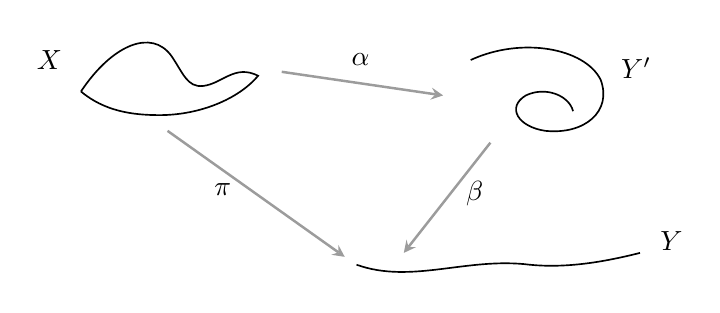
\begin{tikzpicture}[x=1cm,y=1cm,>=stealth,line width=0.5pt]
\draw[line width=0.6pt] (-0.6,0.55) .. controls (-0.2,1.15) and (0.3,1.35) .. (0.55,1.0)
      .. controls (0.7,0.78) and (0.75,0.6) .. (0.95,0.62)
      .. controls (1.2,0.65) and (1.35,0.9) .. (1.65,0.75)
      .. controls (1.4,0.45) and (0.9,0.25) .. (0.4,0.25)
      .. controls (0.05,0.25) and (-0.3,0.3) .. (-0.6,0.55);
\node at (-1.0,0.95) {$X$};
\draw[line width=0.6pt] (4.35,0.95) .. controls (5.0,1.25) and (5.8,1.1) .. (6.0,0.7)
      .. controls (6.15,0.3) and (5.8,0.0) .. (5.3,0.05)
      .. controls (4.95,0.1) and (4.8,0.35) .. (5.05,0.5)
      .. controls (5.3,0.62) and (5.6,0.5) .. (5.65,0.3);
\node at (6.45,0.85) {$Y'$};
\draw[line width=0.6pt] (2.9,-1.65) .. controls (3.6,-1.9) and (4.3,-1.55) .. (5.1,-1.65)
      .. controls (5.6,-1.7) and (6.1,-1.6) .. (6.5,-1.5);
\node at (6.9,-1.35) {$Y$};
\draw[->,gray!70!black!60,line width=0.9pt] (1.95,0.8) -- (4.0,0.5);
\node at (2.95,0.95) {$\alpha$};
\draw[->,gray!70!black!60,line width=0.9pt] (0.5,0.05) -- (2.75,-1.55);
\node at (1.2,-0.7) {$\pi$};
\draw[->,gray!70!black!60,line width=0.9pt] (4.6,-0.1) -- (3.5,-1.5);
\node at (4.4,-0.75) {$\beta$};
\end{tikzpicture}
\caption{\trStein{}因子分解。（依原书手绘图重绘。）}
\label{fig:stein-factorization}
\end{figure}

如常，\trNoether{}假设可以去掉（见 [Stacks, tag 03H2]）。

\emph{\mbox{\trStein{}因子分解定理~28.4.3} 的证明。}\quad 由\mbox{\trGrothendieck{}凝聚定理~18.9.1}，$\pi_*\OO_X$ 是 $Y$ 上的一个\trCoherentSheaf（\trSheafOfAlgebras）。令 $Y':=\Spec\pi_*\OO_X$，于是（由于 $\pi_*\OO_X$ 是\trFiniteType{}的）\trStructureMorphism{} $\beta\colon Y'\to Y$ 是有限的。我们有一个因子分解
\[
\begin{tikzcd}[row sep=2.8em, column sep=4.5em]
X \ar[rr, "\alpha"'] \ar[dr, "\pi"'] && {Y'} \ar[dl, "\beta", "\text{finite}"'] \\
& Y &
\end{tikzcd}
\]
由针对\trProper\trMorphism{}的\mbox{\trCancellationTheorem~11.1.1}，$\alpha$ 是\trProper{}的。最后，我们证明 $\alpha$ 是 $\OO$-连通的，也就是说，$\OO_{Y'}\to\alpha_*\OO_X$ 是一个\trIsomorphism。由于 $\beta$ 是仿射\trMorphism（从而 $\beta_*$ 是从 $\mathit{Coh}_{Y'}$ 到 $\mathit{Coh}_Y$ 的一个\trExact\trFunctor），所以施以前推 $\beta_*$ 之后再作检验就足够了。但 $\beta_*\OO_{Y'}\to\beta_*\alpha_*\OO_X$ 就是恒等映射 $\pi_*\OO_X\to\pi_*\OO_X$（这里我们用到 $\beta_*\OO_{Y'}=\pi_*\OO_X$——见 \S17.1.4——以及 $\beta_*\alpha_*\OO_X=\pi_*\OO_X$）。\hfill$\square$

\textbf{28.4.B.（练习）}\quad 设 $\pi\colon X\to Y$ 是不可约\trVariety{}之间的一个\trProper{}、\trBirational{}\trMorphism。再设 $Y$ 是\trNormal{}的。证明：$\pi$ 是 $\OO$-连通的。（例如，这适用于沿光滑\trCenter{}对光滑\trVariety{}作\trBlowup{}的情形。）于是，由\mbox{\trZariski{}连通性引理~28.4.1}，$\pi$ 具有\trConnected{}的\trFiber。这被称为\mbox{\trZariskiMainTheorem}（双有理\trMorphism{}的版本）。提示：\mbox{练习~10.7.P}。

\textbf{28.4.C.（练习）}\quad 设 $\pi\colon X\to Y$ 与 $\pi'\colon X\to Y'$ 是整的局部\trNoether{}\trScheme{}之间的两个\trProper{}、\trBirational{}\trMorphism，各自把 $X$ 的同一个\trConnected{}集合收缩为一点（而在其余之处是\trIsomorphism），并设 $Y$ 与 $Y'$ 都是\trNormal{}的。证明：$\pi$ 与 $\pi'$ 是相同的\trMorphism（或更确切地说：存在\trIsomorphism{} $i\colon Y\xrightarrow{\ \sim\ }Y'$ 使得 $\pi'=i\circ\pi$）。非正式的转述：若 $X\to Y$ 具有\trConnected{}的\trFiber，那么仅凭知道 $X$ 上被收缩的\trLocus，$Y$ 就被确定了。提示：先把 $Y$ 与 $Y'$ 作为\trTopologicalSpace{}等同起来，再把 $\pi$ 与 $\pi'$ 作为\trTopologicalSpace{}之间的映射等同起来。用\trStein{}因子分解去复原作为 $\pi_*\OO_X$ 的\trStructureSheaf。

\textbf{28.4.D.（练习）}\quad 证明：局部\trNoether{}\trScheme{}之间的\trMorphism{} $\pi\colon X\to Y$ 的\trStein{}因子分解的构造，与局部\trNoether{}\trScheme{}之间的任何\trFlat\trBaseChange{} $Z\to Y$ 相交换。

\textbf{28.4.4. \trCurve{}的\trResolutionOfSingularities。}

若 $C$ 是域 $k$ 上的一条既约\trProjective\trCurve，那么我们可以通过\trNormalization{}来解消它的奇点：$\nu\colon\tilde{C}\to C$。（关于\trResolutionOfSingularities{}的一些讨论见\mbox{注记~22.4.6}；正规\trCurve{}是\trRegular{}的理由见\mbox{定理~13.5.8}。）但从诸例子中我们已经看到，想弄清如何取\trIntegralClosure{}既需要运气也需要洞察力，而我常常两者皆无。我们现在要通过解释如何用\trBlowup{}去奇点，来除掉去奇点过程中的（需要灵感的）猜测成分。算法很简单：我们找到一个\trSingularPoint，把它胀开，然后再寻找更多的\trSingularPoint{}来重复这一过程。显然，如果找不到\trSingularPoint{}了，我们就完工了；问题在于要证明这一过程保证会终止。我们靠利用一个整数不变量来做到这一点：\trArithmeticGenus。我们必须证明：(i) 若 $p_a(\tilde{C})=p_a(C)$，则 $\nu$ 是一个\trIsomorphism——$\tilde{C}$ 已经是非奇异的；(ii) 若 $C'\to C$ 是一个\trBirational\trMorphism，则 $p_a(C')\le p_a(C)$（于是 $p_a(\tilde{C})$ 将是整个过程中\trArithmeticGenus{}的一个下界）；以及 (iii) 胀开一个\trSingularPoint{}会使\trArithmeticGenus{}下降。

为建立这些结果，我们考虑如下的情境。设 $\pi\colon C'\to C$ 是一个\trFinite\trMorphism（其中 $C$ 如上一段所述，而 $C'$ 是一条既约\trCurve），它在 $C$ 的一个有限闭子集之外是\trIsomorphism（从而 $\pi$ 是\trBirational{}的）。于是，拉回映射 $\OO_C\to\pi_*\OO_{C'}$ 没有核，因为 $C$ 是既约的；而且该映射在 $C$ 的各分量的一般点处是\trIsomorphism。其余核 $\mathscr{G}$ 的\trSupport{}落在由有限个\trClosedPoint{}组成的集合上，于是对 $i>0$ 有 $\mathrm{H}^i(C,\mathscr{G})=0$；并且若 $\mathrm{H}^0(C,\mathscr{G})=0$，则 $\mathscr{G}=0$。从正合列
\[
0\longrightarrow\OO_C\longrightarrow\pi_*\OO_{C'}\longrightarrow\mathscr{G}\longrightarrow 0,
\]
以及 $\pi$ 为仿射这一事实，可得 $\chi(C',\OO_{C'})=\chi(C,\OO_C)+\chi(C,\mathscr{G})$，从而 $p_a(C)\ge p_a(C')$，而等号成立当且仅当 $\pi$ 是 $\OO$-连通的（即 $\mathscr{G}=0$）。

\textbf{28.4.E.（练习）}\quad 证明：若 $\pi$（如上）是 $\OO$-连通的，则 $\pi$ 是一个\trIsomorphism。提示：证明仿射的 $\OO$-连通\trMorphism{}都是\trIsomorphism。

为完成我们的策略，还剩一件事要证：若 $\beta\colon C'\to C$ 是 $C$ 在一点 $p$ 处的\trBlowup，而 $\beta$ 是一个\trIsomorphism，则 $C$ 在该点处已经是非奇异的。但如果 $\beta$ 是\trIsomorphism，那么 $p$ 就是\trExceptionalDivisor，从而是一个\trEffectiveCartierDivisor，从而局部地由单个方程\footnote{原书此处作「a singular equation」，按文义当为「a single equation」之误（single 误排作 singular），径改。——译者注}截出。但这样一来，$\mathfrak{m}_{C,p}\subset\OO_{C,p}$ 就是\trPrincipal{}的，故 $\OO_{C,p}$ 是一个维数为 $1$ 的\trRegular\trLocalRing。

（你应当核实一下：我们确实完成了我们的策略。你能把这个论证推广到 $C$ 非\trProjective{}的情形吗？）

曲面的\trResolutionOfSingularities{}将在 \S28.6.4 中简略讨论。


\section{\trZariskiMainTheorem}

\trZariskiMainTheorem{}这个名称在一切可能的方面都取错了（虽然还不算错得可怕）。它并不是单独某一条\emph{定理}，因为以这个名字流传的结果有很多，而且它们往往显得彼此毫不相干。它们的共同之处在于：它们都是 \trZariski{}某条特定结果在思想上的后裔。而这条结果并不是 \trZariski{}那多产生涯中的\emph{主}定理；这个名字的来由，不过是它作为某篇具体论文 [Z] 的「主定理」罢了。最后，它也谈不上在比这更强的意义上「属于 \trZariski」；现代的诸版本都出自 \trGrothendieck{}之手。
我们已经见过\trZariskiMainTheorem{}的一个版本：\mbox{练习~28.4.B} 的「\trBirational」形式。本节的目标是证明一个更强的陈述，它已十分接近最优的版本。
在开始之前，我们指出：一个\trProper\trMorphism{}在一点 $q\in Y$ 之上的\trFiber{}是\trResidueField{} $\kappa(q)$ 上的一个\trProper{}（从而\trFiniteType）的\trScheme；而若一个点构成该\trFiber{}的一个\trDimension{}为 $0$ 的分量，我们就说它\textbf{在其\trFiber{}中孤立}（isolated in its fiber）。（这里的「分量」兼指\trConnectedComponent{}与\trIrreducibleComponent。）

\textbf{28.5.1. \trZariskiMainTheorem（\trGrothendieck{}形式）。}\ ——\ \emph{设 $\pi\colon X\to Y$ 是局部\trNoether{}\trScheme{}之间的一个\trProper\trMorphism。}

\emph{(a) $X$ 中在其\trFiber{}中孤立的那些点构成一个\trOpenSubset{} $X_0\subset X$。}

\emph{(b) \trMorphism{} $\pi|_{X_0}\colon X_0\to Y$ 可分解为一个\trOpenEmbedding{} $X_0\hookrightarrow Y'$，随后接一个\trFinite\trMorphism{} $Y'\to Y$。}

\emph{(c) \trMorphism{} $\pi\colon X\to Y$ 经由 $Y'$ 分解。}

\begin{equation*}
\tag{28.5.1.1}\label{eq:zmt-factorization}
\begin{tikzcd}[row sep=2.6em, column sep=3.2em]
 & X \ar[dr, "\alpha"] \ar[dd, bend right=15, "\pi"'] & \\
X_0 \ar[ur, hook, "\text{open}"] \ar[rr, hook, bend right=12, "\text{open}"] \ar[dr, "\pi|_{X_0}"'] && Y' \ar[dl, "\beta", "\text{finite}"] \\
 & Y &
\end{tikzcd}
\end{equation*}

与\trStein{}因子分解一样，定理的证明所给出的是一个\emph{特定的}因子分解。事实上，$X\to Y'=\Spec\pi_*\OO_X\to Y$ 正是 $\pi\colon X\to Y$ 的\trStein{}因子分解，由此 (c) 与 (b) 的一部分便基本上立即可得。
若 $\pi$ 是\emph{\trVariety}之间的\trMorphism，那么由\trFiber\trDimension{}的\trUpperSemicontinuous{}性（\mbox{定理~12.4.3(a)}），我们其实已经知道 (a) 部分。因此，\trVariety{}情形的证明要更容易些，而且（即便你感兴趣的正是更一般的情形）我们也建议你在阅读证明时把它限制在这个较简单的情形上，以便专注于主要思想。但即便在\trVariety{}的情形，我们也会需要 (a) 的证明中产生的某些想法，所以你应当把它一直读到被告知可跳往 (b) 之处为止。
\emph{证明。}\quad (a) 取 $\pi$ 的\trStein{}因子分解 \eqref{eq:stein-factorization-triangle}：
\[
\begin{tikzcd}[row sep=2.8em, column sep=4.5em]
X \ar[rr, "\text{$\OO$-conn.}", "\alpha"'] \ar[dr, "\pi"'] && Y' \ar[dl, "\beta", "\text{finite}"'] \\
& Y &
\end{tikzcd}
\]
由于 $\beta$ 是\trFinite{}的，$X$ 的一个点是 $\pi$ 的\trFiber{}中的孤立点，当且仅当它是 $\alpha$ 的\trFiber{}中的孤立点。于是我们可以用 $\alpha$ 代替 $\pi$。（基本上，我们是在化归到「$\pi$ 为 $\OO$-连通」的情形，但我们宁愿谨慎地把当前考虑的\trMorphism{}称作 $\alpha$，以便 (b) 的证明中还能回到对 $\pi$ 的讨论。）
由于局部\trNoether{}\trScheme{}之间的\trProper{}、$\OO$-连通\trMorphism{}的诸\trFiber{}都是\trConnected{}的（\mbox{\trZariski{}连通性引理~28.4.1}），一个点在 $\alpha$ 的\trFiber{}中孤立，当且仅当它\emph{就是}整条\trFiber。
如果你只考虑\trVariety{}情形，那么此时你应当直接跳到 (b) 部分的证明。
为证 $X_0$ 是\trOpen{}的，我们将把它等同于 $\Omega_\alpha=0$ 的\trLocus（即 $\alpha$ 的\trUnramified\trLocus——注意不是 $\pi$ 的！），由\mbox{练习~21.7.H}，它是\trOpen{}的。

\textbf{28.5.A.（练习）}\quad 若 $\Omega_\alpha|_p=0$，证明：$p$ 在 $\alpha$ 的\trFiber{}中孤立（从而也在 $\pi$ 的\trFiber{}中孤立）。

现在我们来证另一个方向。设 $p$ 在它的\trFiber{}中孤立，并设 $r\in Y'$ 为 $\alpha(p)$。我们将证明：$\alpha$ 诱导出一个\trIsomorphism{} $\alpha^{\sharp}\colon\OO_{Y',r}\xrightarrow{\ \sim\ }\OO_{X,p}$，从而 $\Omega_{\OO_{X,p}/\OO_{Y',r}}=0$。由于 $\Omega$ 的构造对源与靶的局部化都有良好的表现（\mbox{练习~21.2.L}），这就蕴含 $(\Omega_\alpha)_p=0$，于是 $\Omega_\alpha$ 在 $p$ 处为 $0$。
\trStalk{} $\OO_{Y',r}$ 的取法是：对 $Y'$ 的所有包含 $r$ 的\trOpenSubset，取（$\OO_{Y'}$ 的\trSection{}的）\trColimit。对任何这样一个\trOpenSubset{} $V\subset Y'$，条件 $\alpha_*\OO_X=\OO_{Y'}$ 给出\trIsomorphism{} $\Gamma(V,\OO_{Y'})\xrightarrow{\ \sim\ }\Gamma(\alpha^{-1}(V),\OO_X)$（与包含关系相容）。我们将证明：由诸 $\alpha^{-1}(V)$（$V$ 遍历 $r$ 的诸\trOpen\trNeighborhood）构成的系统——其每一员都必然包含 $p$——与 $p$ 在 $X$ 中的\trOpen\trNeighborhood{}系统共尾。为此，我们必须证明：对 $p$ 在 $X$ 中的任何\trOpen\trNeighborhood{} $U$，都存在 $r$ 在 $Y'$ 中的\trOpen\trNeighborhood{} $V$，使得 $\alpha^{-1}(V)\subset U$。为此，注意 $X\setminus U$ 在 $X$ 中是\trClosed{}的，故 $\alpha(X\setminus U)$ 在 $Y'$ 中是\trClosed{}的（因为 $\alpha$ 是\trProper{}的），于是其\trComplement{} $V:=Y'\setminus\alpha(X\setminus U)$ 是\trOpen{}的。但 $\alpha^{-1}(V)\subset U$，如此便证得所需。

(b)（\emph{\trSet}）在对 (a) 的证明中，我们已经确立：$\alpha$ 在 $X_0$ 与 $Y'$ 的一个\trOpenSubset{}之间给出一个\trBijection。

（\emph{\trTopology}）我们基本上也已经证明：$\alpha$ 给出一个\trHomeomorphism。$Y'$ 的任何\trOpenSubset{}由 $\alpha$ 的\trContinuous{}性拉回为 $X_0$ 的一个\trOpenSubset；而若 $U$ 是 $X_0$ 的一个\trOpenSubset，则 $\alpha(X\setminus U)$ 是 $Y'$ 的一个\trClosedSubset，于是它的\trComplement（即 $\alpha(U)$，这里用到\trProper{}的 $\OO$-连通\trMorphism{}皆为\trSurjectiveMap{}的这一事实，\mbox{练习~25.1.H}）是\trOpen{}的。

（\emph{\trSheaf}）利用这个\trTopologicalSpace{}之间的\trIsomorphism，$\alpha$（限制在 $\alpha(X_0)$ 上）的 $\OO$-连通性表明：$\alpha$ 给出\trLocallyRingedSpace（即\trScheme）之间的一个\trIsomorphism{} $X_0\to\alpha(X_0)$。

这样，我们就找到了想要的因子分解。（(c) 部分由我们的构造立即可得。）\hfill$\square$

\textbf{28.5.B.（练习）}\quad 在稍有不同的假设下证明\trZariskiMainTheorem：设 $Y$ 是\trAffine{}的，比如说 $\Spec A$，而 $X$ 是一个\trQuasiprojective{} $A$-\trScheme。（提示：由\trQuasiprojective{} $A$-\trScheme{}的\mbox{定义~4.5.10}，我们可以找到一个\trOpenEmbedding{} $X\hookrightarrow X'$，其中 $X'$ 是一个\trProjective{} $A$-\trScheme。将\mbox{定理~28.5.1} 施于 $X'\to\Spec A$。）
作为\trZariskiMainTheorem{}的一个应用，我们终于可以证明那个我们已多次提及的、关于\trFinite\trMorphism{}的刻画。

\textbf{28.5.2. \trhTheorem。}\ ——\ \emph{设 $\pi\colon X\to Y$ 是局部\trNoether{}\trScheme{}之间的一个\trMorphism。则下列诸条等价。}

\emph{(a) $\pi$ 是\trFinite{}的。}

\emph{(b) $\pi$ 是\trAffine{}且\trProper{}的。}

\emph{(c) $\pi$ 是\trProper{}且\trQuasifinite{}的。}

如常，\trNoether{}假设可以去掉：[Gr-EGA, IV$_3$.8.11.1] 表明，\trProper、\trQuasifinite、\trLocally\trFinitelyPresented{}的\trMorphism{}都是\trFinite{}的。

\emph{证明。}\quad \trFinite\trMorphism{}依定义是\trAffine{}的，且由\mbox{命题~11.4.3} 是\trProper{}的，故 (a) 蕴涵 (b)。
为证 (b) 蕴涵 (c)，我们只需证明\trAffine{}的\trProper\trMorphism{}具有\trFinite\trFiber（因为\trQuasifinite{}性定义中「\trFiniteType」的那一部分已由\trProper{}性替我们办妥）。这一点已在\mbox{练习~18.9.A} 中证得。
最后，我们假设 (c)，即 $\pi$ \trProper{}且\trQuasifinite，并来证明 (a)，即 $\pi$ 是\trFinite{}的。由\mbox{\trZariskiMainTheorem~28.5.1}，我们有一个因子分解 \eqref{eq:zmt-factorization}：
\[
\begin{tikzcd}[row sep=2.8em, column sep=4.5em]
X_0 \ar[rr, hook, "\text{open}", "\gamma"'] \ar[dr, "\pi"'] && Y' \ar[dl, "\text{finite}"] \\
& Y &
\end{tikzcd}
\]
现在 $X=X_0$。（你看出这是为什么吗？提示：先\mbox{练习~8.4.D}，后\mbox{练习~8.3.G}。）由针对\trProper\trMorphism{}的\mbox{\trCancellationTheorem~11.1.1}（用到 $Y'\to Y$ 是\trFinite{}的从而\trSeparated），$\gamma$ 是\trProper{}的。

\textbf{28.5.C.（练习）}\quad 证明：\trProper{}且\trQuasicompact{}的\trOpenEmbedding{}都是\trClosedEmbedding。提示：利用\mbox{推论~9.4.5}（对\trQuasicompact{}\trMorphism，像的\trClosure{}就是\trClosure{}的像）来证明其像在靶中既\trOpen{}又\trClosed。

把这条结论施于我们的情势，我们看到 $X\to Y$ 是两个\trFinite\trMorphism{} $\gamma\colon X\hookrightarrow Y'$ 与 $Y'\to Y$ 的复合，从而其自身是\trFinite{}的。\hfill$\square$

\textbf{28.5.3.}\ \emph{\trNagata{}紧化定理。}\quad 对于最后两个应用（\mbox{练习~28.5.E} 与\mbox{练习~28.5.F}），我们需要一个恼人的假设，而上一道练习恰好为它作了预演。设 $\pi\colon X\to Y$ 是局部\trNoether{}\trScheme{}之间的一个\trMorphism。若对 $Y$ 的某个\trOpenCover{}中的一切\trAffine\trOpenSet{} $U_i$，限制 $\pi|_{\pi^{-1}(U_i)}\colon\pi^{-1}(U_i)\to U_i$ 都能分解为一个\trOpenEmbedding{}，嵌入到某个在 $U_i$ 上\trProper{}的\trScheme{}之中，我们就说 $\pi$ 满足 $(\dagger)$。满足 $(\dagger)$ 的\trMorphism{}必是\trSeparated{}且\trFiniteType{}的。事实证明这个条件已经足够：\textbf{\trNagata{}紧化定理}（Nagata's Compactification Theorem）断言，\trNoether{}\trScheme{}之间的\emph{每一个}\trSeparated{}且\trFiniteType{}的\trMorphism{} $\pi\colon X\to Y$ 都可以分解为一个\trDense\trOpenEmbedding{}，嵌入到某个在 $Y$ 上\trProper{}的\trScheme{}之中。（证明见 [Lüt]。\trNoether{}假设可以换成「$Y$ 为\trQuasicompact{}且\trQuasiSeparated{}」这一条件，见 [Con]。）

\textbf{28.5.D.（练习）}\quad 证明：若 $\pi\colon X\to Y$ 是 $k$ 上的\trVariety{}之间的一个\trMorphism，而 $X$ 是某个\trProper\trVariety{} $Z$ 的一个\trOpenSubset，则 $\pi$ 满足 $(\dagger)$。（提示：$X$ 是它在 $Z\times_k Y$ 中的\trClosure{}的一个\trOpenSubscheme。）

\textbf{28.5.E.（练习）}\quad 设 $\pi\colon X\to Y$ 是整的局部\trNoether{}\trScheme{}之间的一个\trQuasifinite{}、\trBirational{}\trMorphism，且 $Y$ 是\trNormal{}的。再设 $\pi$ 满足 $(\dagger)$。证明：$\pi$ 是一个\trOpenEmbedding。（于是，若进而 $\pi$ 还是\trBijection，则 $\pi$ 必是\trIsomorphism。）提示：「是\trOpenEmbedding」这一条件在靶上是局部的。

\textbf{28.5.F.（练习）}\quad 设 $\pi\colon X\to Y$ 是\trNoether{}\trScheme{}之间的一个\trSeparated、\trQuasifinite\trMorphism。

(a) 假设\trNagata{}紧化定理（\S28.5.3）成立，证明：$\pi$ 可分解为一个\trOpenEmbedding{}，嵌入到一个\trFinite\trMorphism{}之中。
\[
\begin{tikzcd}[row sep=2.8em, column sep=4.5em]
X \ar[rr, hook, "\text{open}"] \ar[dr, "\pi"'] && Y' \ar[dl, "\text{finite}"] \\
& Y &
\end{tikzcd}
\]

(b) 改为假设 $\pi$ 满足 $(\dagger)$，证明：$\pi$ 「局部地」分解为一个\trOpenEmbedding{}，嵌入到一个\trFinite\trMorphism{}之中；也就是说，存在 $Y$ 的一个\trOpenCover{} $U_i$\footnote{原书此处作「a open cover」，当为「an open cover」之误，径改。——译者注}，使得在每个 $U_i$ 之上都有这样一个因子分解。

这印证了把\trQuasifinite\trMorphism{}看作「\trFinite\trMorphism{}的\trOpenSubset」的想法，如 \S8.3.12 中所许诺的那样。

\textbf{28.5.4.}\ \extrahard\ \textbf{其他版本的\trZariskiMainTheorem。}

\mbox{定理~28.5.1} 中的\trNoether{}条件可以放宽（见 [Stacks, tag 02LQ]、[Gr-EGA, IV$_3$.8.12.13] 或 [GW, Thm. 12.73]）：若 $\pi\colon X\to Y$ 是一个\trSeparated{}且\trFiniteType{}的\trMorphism，而 $Y$ 是\trQuasicompact{}且\trQuasiSeparated{}的，则在其\trFiber{}中孤立的点集 $X_0$ 在 $X$ 中是\trOpen{}的，并且对 $X_0$ 的每个\trQuasicompact{}的\trOpenSubset{} $U$，都有一个因子分解
\[
\begin{tikzcd}[row sep=2.8em, column sep=4.5em]
U \ar[rr, "\gamma"] \ar[dr, "\pi|_U"'] && Y' \ar[dl, "\beta"', "\text{finite}"] \\
& Y &
\end{tikzcd}
\]
使得 $\beta$ 是\trFinite{}的，$\gamma|_U$ 是一个\trQuasicompact{}的\trOpenEmbedding，并且满足 $\gamma^{-1}(\gamma(U))=U$。
此外还有\trZariskiMainTheorem{}的拓扑形式与幂级数形式，见 [Mu7, \S III.9]。


\section{收缩 $(-1)$-\trCurve{}的\trCastelnuovo{}判别准则}

我们在\mbox{练习~22.4.O} 中已经看到：在一张\trRegular\trSurface{}的一个（既约）点处作\trBlowup，所得的\trExceptionalDivisor{}是一条 $(-1)$-\trCurve{}（见\mbox{定义~20.2.8}：它\trIsomorphic{}于 $\mathbb{P}^1$，且其\trNormalBundle{}为 $\OO_C(-1)$）。\trCastelnuovo{}判别准则是它的逆命题：若我们有一张含有 $(-1)$-\trCurve{}的\trQuasiprojective{}\trSurface，那么这张曲面就是在另一张曲面的一个既约正则点处作\trBlowup{}得到的。我们就说这条 $(-1)$-\trCurve{}可以被\textbf{收缩}（blow down）。
\textbf{28.6.1. \trhTheorem（\trCastelnuovo{}判别准则）。}\ ——\ \emph{设 $C\subset X$ 是 $k$ 上一张\trSmooth\trProjective{}\trSurface{}上的一条 $(-1)$-\trCurve。则存在一个\trBirational\trMorphism{} $\pi\colon X\to Y$，使得 $Y$ 是一张\trSmooth\trProjective{}\trSurface，$\pi(C)$ 是一个 $k$-\trValuedPoint，$\pi$ 是 $Y$ 在该点处的\trBlowup，而 $C$ 是这次\trBlowup{}的\trExceptionalDivisor。}
由\mbox{练习~28.4.C}，「收缩 $C$」的办法只有一种：这个收缩是唯一的。
\emph{证明。}\quad 证明分三步。\emph{第 1 步.} 我们构造 $\pi\colon X\to Y$，它把 $C$ 收缩为一点 $q$（且在其余之处是\trIsomorphism）。到这一步完成时，我们将知道 $Y$ 是一个\trProjective\trVariety。\emph{第 2 步.} 然后我们证明 $Y$ 是\trSmooth{}的；这是最艰难的一步，需要用到\mbox{形式函数定理~28.3.2}。\emph{第 3 步.} 最后，我们认出 $\pi$ 就是\trBlowup{} $\mathrm{Bl}_q\,Y\to Y$。
\emph{第 1 步.}\quad 我们的思路是找出一个\trInvertibleSheaf{} $\mathscr{L}$，让它的完全线性系来承担这项任务。我们从 $X$ 上一个满足 $\mathrm{H}^1(X,\mathscr{H})=0$ 的\trVeryAmple\trInvertibleSheaf{} $\mathscr{H}$ 出发。这样的\trInvertibleSheaf{} $\mathscr{H}$ 可以如下找到：任取一个\trVeryAmple\trInvertibleSheaf，再取其一个适当大的倍数，其间援引\mbox{练习~16.2.C}（\trVeryAmple{} $\otimes$ \trVeryAmple{} $=$ \trVeryAmple{}）与\trSerre{}消失（\mbox{定理~18.1.3}~(ii)）。令 $d=\mathscr{H}\cdot C:=\deg_C\mathscr{H}|_C$。由 $\mathscr{H}$ 的\trVeryAmpleness{}（\mbox{练习~20.1.K}）可知 $d>0$。
\textbf{28.6.A.（练习）}\quad 证明：$\mathrm{H}^1(X,\mathscr{H}(iC))=0$（$0\le i\le d$）。提示：对 $i$ 作归纳，利用
\begin{equation*}
\tag{28.6.1.1}\label{eq:castelnuovo-restriction-seq}
0\longrightarrow\mathscr{H}((i-1)C)\longrightarrow\mathscr{H}(iC)\longrightarrow\mathscr{H}(iC)|_C\longrightarrow 0.
\end{equation*}
提示：注意 $\mathscr{H}(iC)|_C$ 是 $C\cong\mathbb{P}^1$ 上的一个\trLineBundle；它是哪一个 $\OO(n)$？
令 $\mathscr{L}:=\mathscr{H}(dC)$。我们将经由映射 $\phi\colon\mathrm{H}^0(X,\mathscr{H})\to\mathrm{H}^0(X,\mathscr{H}(dC))$，用 $\mathscr{H}$ 的\trSection{}来得到 $\mathscr{L}$ 的\trSection。
\textbf{28.6.B.（练习）}\quad 证明：$\mathscr{L}$ 是\trBasePointFree{}的。提示：要证明 $\mathscr{L}$ 在 $C$ 之外没有基点，考虑 $\phi$ 的像。要证明 $\mathscr{L}$ 在 $C$ \emph{上}没有基点，则利用：由 \eqref{eq:castelnuovo-restriction-seq}，当 $i=d$ 时，$\mathrm{H}^0(X,\mathscr{L})\to\mathrm{H}^0(C,\mathscr{L}|_C)$ 是满射，并且 $\mathscr{L}|_C\cong\OO_C$。
于是，完全线性系 $|\mathscr{L}|$ 给出一个从 $X$ 到某个\trProjectiveSpace{} $\mathbb{P}^N$ 的\trMorphism{} $\pi'$。
\textbf{28.6.C.（练习）}\quad 证明：$\pi'$ 恰好把 $C$ 收缩为一点 $q'$。更明确地说，证明：$\pi'$ 把 $C$ 送到一点 $q'$，而 $\pi'|_{X\setminus C}\colon X\setminus C\to\mathbb{P}^N\setminus\{q'\}$ 是一个\trClosedEmbedding。提示：要证明 $\pi'$ 在 $C$ 之外给出一个\trClosedEmbedding，注意 $|\mathscr{H}|$ 分离点与切向量，并论证 $|\mathscr{L}|=|\mathscr{H}(dC)|$ 在 $C$ 之外分离点与切向量。要证明 $C$ 被 $\pi'$ 收缩，则利用 $\deg\mathscr{L}|_C=0$ 这一事实。
令 $Y'$ 为 $\pi'$ 的像，于是我们有一个\trMorphism{} $X\to Y'$（我们也称它为 $\pi'$）。令 $\nu\colon Y\to Y'$ 为 $Y'$ 的\trNormalization，于是由正规化的\trUniversalProperty{}（\S10.7），$\pi'$ 提升为 $\pi\colon X\to Y$。（我们作正规化，是为了能在第 2 步中用上\mbox{练习~28.4.B}。）
\textbf{28.6.D.（容易练习）}\quad 证明：$\nu^{-1}(q')\subset Y$ 是单独一个点，我们把它称作 $q$，并且 $\pi(C)=q$。（提示：$\pi$ 的像是\trClosed{}的，而 $\pi(C)$ 是\trConnected{}的。）
\textbf{28.6.E.（练习）}\quad 设 $X$ 是一张\trSmooth\trProjective{}\trSurface，含有一条\trIsomorphic{}于 $\mathbb{P}^1_k$ 的\trCurve{} $C\subset X$。若 $C\cdot C:=\deg_C\OO(C)|_C<0$，证明：存在一个\trMorphism{} $\pi\colon X\to X'$，它把 $C$ 收缩为一点，而让 $X$ 的其余部分保持不变。（这条练习不会被用到，收在这里是为了让人练习第 1 步中的论证。）
\emph{第 2 步.}\quad 现在我们来证明 $Y$ 是一张\trSmooth\trSurface。由于 $Y$ 是\trNormal{}的，由\mbox{练习~28.4.B}，我们有 $\pi_*\OO_X\cong\OO_Y$（即 $\pi\colon X\to Y$ 是 $\OO$-连通的）。我们将这样来证明 $Y$ 在 $q$ 处\trSmooth：证明作为拓扑环有 $\hat{\OO}_{Y,q}\cong k[[x,y]]$，因为这样一来便有 $\dim_k(\mathfrak{m}/\mathfrak{m}^2)=2$。（你明白为什么这就表明 $Y$ 是\trSmooth{}的，而不仅仅是\trRegular{}的吗？）由\mbox{形式函数定理~28.3.2}，$\hat{\OO}_{Y,q}\cong\lim_{n\to\infty}\mathrm{H}^0(C'_n,\OO_{C'_n})$，其中 $C'_n$ 是 $X$ 的这样一个\trClosedSubscheme：它是 $q$ 的 $n$ 阶形式邻域的\trSchemeTheoreticPreimage。
我们并不确切知道这个 $n$ 阶形式邻域是什么，但这无妨：这个逆向系统与 $\OO(-nC)=\mathscr{I}^n_{C/X}$ 共尾（你看出是为什么吗？），所以我们可以改取后者的\trInverseLimit{}（据\mbox{练习~28.1.A}）。只须证明：对一切 $n\ge 0$ 都有 $\mathrm{H}^0(C_n,\OO_{C_n})\cong k[[x,y]]/(x,y)^n$，其中 $C_n$ 由下式定义
\[
0\longrightarrow\OO(-nC)\longrightarrow\OO_X\longrightarrow\OO_{C_n}\longrightarrow 0.
\]
（当心：我们并不知道 $C_n=C'_n$，甚至连 $C_1=C'_1$ 也不知道。就我们所知，$q$ 之上的\trFiber{}完全可能是非既约的！）
我们按 $n$ 归纳来证。作为 $k$-\trVectorSpace{}这很容易，只需利用
\begin{equation*}
\tag{28.6.1.2}\label{eq:castelnuovo-graded-piece-seq}
0\longrightarrow\mathscr{I}^n/\mathscr{I}^{n+1}\longrightarrow\OO_{C_{n+1}}\longrightarrow\OO_{C_n}\longrightarrow 0
\end{equation*}
（即 $C_n$ 在 $C_{n+1}$ 中的\trClosedSubscheme{}正合列 \eqref{eq:closed-subscheme-exact-sequence}），并利用典范\trIsomorphism{} $\mathrm{H}^0(\mathbb{P}^1,\OO_{\mathbb{P}^1}(n))\stackrel{\sim}{\hookrightarrow}\Sym^n\bigl(\mathrm{H}^0(\mathbb{P}^1,\OO_{\mathbb{P}^1}(1))\bigr)$。棘手之处在于：我们要的这个同构是作为\emph{环}的同构。
\textbf{28.6.F.（练习）}\quad 证明这一点。（这可能让你回想起，我们曾在\mbox{练习~19.11.E} 中求出一个\trInvertibleSheaf{}的\trTotalSpace{}上的函数环。这并非巧合。）提示：把 $\mathscr{I}^n/\mathscr{I}^{n+1}$ 解读为 $\Sym^n(\mathscr{I}/\mathscr{I}^2)$（\mbox{推论~22.3.9}），进而把它解读为 $\OO_{\mathbb{P}^1}(n)$，并证明：取整体\trSection{}之后，\eqref{eq:castelnuovo-graded-piece-seq} 仍然正合。到这里，你将已经证明：$\mathrm{H}^0(C_n,\OO_{C_n})$ 的某种\trAssociatedGraded{}环同构于 $k[[x,y]]/(x,y)^n$。请证明这就足以建立所欲求的环同构。
于是我们得到了\trSmooth{}性，第 2 步完成。
\emph{第 3 步.}\quad 现在我们必须认出 $\pi$ 就是 $Y$ 在 $q$ 处的\trBlowup。由于 $C$ 是 $X$ 上的一个\trEffectiveCartierDivisor，由胀开的\trUniversalProperty{}可知\footnote{原书此处作「by the universal property of blowing up means that」，「by $\ldots$」与「means that」两句式杂糅，兹按文义译出。——译者注}，存在唯一的\trMorphism{} $\alpha$ 使下图交换：
\[
\begin{tikzcd}[row sep=2.8em, column sep=4.5em]
X \ar[rr, "\alpha"] \ar[dr, "\pi"'] && \mathrm{Bl}_q\,Y \ar[dl, "\beta"] \\
& Y. &
\end{tikzcd}
\]
由针对\trProjective\trMorphism{}的\trCancellationTheorem{}（\mbox{练习~17.3.C}），$\alpha$ 是\trProjective{}的。
\textbf{28.6.G.（练习）}\quad 证明：$\alpha$ 具有\trFinite\trFiber。
由于具有有限\trFiber{}的\trProjective\trMorphism{}是\trFinite{}的（\mbox{定理~18.1.6}），$\alpha$ 是一个\trFinite\trMorphism。但这样一来，$\alpha$ 是一个到\trNormal\trScheme{}的\trBirational\trFinite\trMorphism，从而由\mbox{练习~10.7.P} 是一个\trIsomorphism。\hfill$\square$
到目前为止，我们只把\mbox{形式函数定理~28.3.2} 用在了 $\mathrm{H}^0$ 上。下一道练习将给你一个机会，看看它在其他\trCohomology{}群上的实际运作。
\textbf{28.6.H.（练习）}

(a) 设 $\beta\colon X=\mathrm{Bl}_q\,Y\to Y$ 是 $k$ 上的一张\trSmooth\trSurface{}在一个\trSmooth{}的 $k$-\trValuedPoint{}处的\trBlowup。证明：$R^1\beta_*\OO_X=R^2\beta_*\OO_X=0$。

(b) 证明：自然映射 $\beta^*\colon\mathrm{H}^1(Y,\OO_Y)\to\mathrm{H}^1(X,\OO_X)$ 与 $\beta^*\colon\mathrm{H}^2(Y,\OO_Y)\to\mathrm{H}^2(X,\OO_X)$ 都是\trIsomorphism。

\textbf{28.6.2. 初等变换。}

回忆\mbox{例~17.2.6} 中给出的\trHirzebruchSurface{} $\mathbb{F}_n$（域 $k$ 上的）的定义。若 $n>0$，则 $\mathbb{F}_n$ 上有唯一一条\trSelfIntersection{}最负的\trCurve{} $E$（\mbox{练习~20.2.R}）。它的\trSelfIntersection{}为 $E\cdot E:=\deg_E\OO(E)|_E=-n$。它是投射 $\pi\colon\mathbb{F}_n\to\mathbb{P}^1$ 的一个\trSection{}。（若 $n=0$，此时 $\mathbb{F}_n\cong\mathbb{P}^1\times\mathbb{P}^1$，则 $E$ 通常被定义为 $\pi\colon\mathbb{P}^1\times\mathbb{P}^1\to\mathbb{P}^1$ 的任意一个「常值」\trSection{}——它并不唯一。）
设 $q$ 是 $\mathbb{F}_n$ 的一个 $k$-\trValuedPoint。令 $F$ 为 $\pi$ 的含有 $q$ 的那条\trFiber。
\textbf{28.6.I.（练习）}\quad 证明：$F\cdot F:=\deg_F\OO(F)|_F=0$。
设 $\beta\colon\mathrm{Bl}_q\,\mathbb{F}_n\to\mathbb{F}_n$ 为在 $q$ 处的\trBlowup，并令 $Z$ 为其\trExceptionalDivisor（因为「$E$」这个名字已被占用）。令 $F'$ 为 $F$ 的\trProperTransform，$E'$ 为 $E$ 的\trProperTransform。
\textbf{28.6.J.（练习）}\quad 证明：$F'\cdot F':=\deg_{F'}\OO(F')|_{F'}=-1$。
于是，由\trCastelnuovo{}判别准则，我们可以把 $F'$ 收缩掉，从而得到一张新的\trSurface{} $Y$。
\textbf{28.6.K.（练习）}\quad 设 $n>0$。若 $q\notin E$，证明：$Y\cong\mathbb{F}_{n-1}$。若 $q\in E$，证明：$Y\cong\mathbb{F}_{n+1}$。可能的提示：倘若你已经知道 $Y$ 是\trHirzebruchSurface{} $\mathbb{F}_m$，那么当 $m>0$ 时，你可以凭借那条唯一具有负\trSelfIntersection{}的\trCurve{}的\trSelfIntersection{}把它认出来。
\textbf{28.6.L.（练习）}\quad 设 $n=0$。证明：$Y\cong\mathbb{F}_1$。提示：\mbox{练习~22.4.K}。
这里的讨论可以推广到更一般的\trCurve{}上的 $\mathbb{P}^1$-丛。下面不过是这个故事的第一步。
\textbf{28.6.M.（练习）}\quad 设 $C$ 是 $k$ 上一条\trSmooth\trCurve，$\pi\colon X\to C$ 是 $C$ 上的一个 $\mathbb{P}^1$-丛。若 $q$ 是 $X$ 的一个 $k$-\trValuedPoint，那么我们可以胀开 $q$，再收缩经过 $q$ 的那条\trFiber{}的\trProperTransform。证明：其结果仍是 $C$ 上的一个 $\mathbb{P}^1$-丛 $X'$。（这称为该\trRuling{}曲面的一个\textbf{初等变换}（elementary transformation）。）
\textbf{28.6.N.（练习）}\quad 设 $X=\mathit{Proj}_C(\mathscr{L}\oplus\mathscr{M})$，而 $q$ 落在相应于正合列
\[
0\longrightarrow\mathscr{L}\longrightarrow\mathscr{L}\oplus\mathscr{M}\longrightarrow\mathscr{M}\longrightarrow 0.
\]
的\trSection{}之上。证明：$X'\cong\mathit{Proj}_C(\mathscr{L}(\pi(q))\oplus\mathscr{M})$。\footnote{原书此处作「$\mathit{Proj}_C(\mathscr{L}(\pi(q))\oplus\mathscr{M}))$」，末尾多出一个右括号，径删。——译者注}
倘若只告诉你 $X\cong\mathit{Proj}_C\,\mathscr{V}$（其中 $\mathscr{V}$ 是一个秩为 $2$ 的\trLocallyFreeSheaf），而 $q$ 落在相应于 \eqref{eq:section-filtration-sequence} 的\trSection{}之上，你能猜测（或者证明）会发生什么吗？

\textbf{28.6.3. 曲面的极小模型。}

代数闭域上的一张\trSurface，若不含 $(-1)$-\trCurve，就称为\textbf{极小的}（minimal）。若\trSurface{} $X$ 不是极小的，我们可以选取一条 $(-1)$-\trCurve{}并把它收缩。若所得\trSurface{}仍不是极小的，我们可以再收缩一条 $(-1)$-\trCurve，如此等等。由\trPicard{}数 $\rho$ 的有限性（这一点我们诚然未曾证明；见 \S18.4.12），再加上收缩会使 $\rho$ 减小 $1$（据\mbox{练习~22.4.O}），这个过程必定终止。由此我们构造出 $X$ 的一个\textbf{极小模型}（minimal model）——一张\trBirational{}于 $X$ 的极小\trSurface。倘若极小模型是唯一的，这便提供了一种按双有理等价给\trSurface{}分类的办法：若 $X$ 与 $X'$ 是\trSmooth\trProjective{}\trSurface，想知道它们是否\trBirational，我们只须找出它们各自的极小模型，再看它们是否\trIsomorphic。
遗憾的是，极小模型并不唯一。$\mathbb{P}^1\times\mathbb{P}^1$ 与 $\mathbb{P}^2$ 的例子表明，同一个双有理等价类中可以有多于一个极小模型。（为什么这两张曲面都是极小的？）此外，$\mathbb{P}^2$ 在两点处的\trBlowup{}与 $\mathbb{P}^1\times\mathbb{P}^1$ 在一点处的\trBlowup{}之间的\trIsomorphism{}（\mbox{练习~22.4.K}）表明，一张\trSmooth\trSurface{}可以拥有多于一个极小模型。
尽管如此，这种不唯一性已被理解得相当透彻：\trZariski{}曾证明，具有多于一个极小模型的\trSurface{}恰是那些\trBirational{}于 $C\times\mathbb{P}^1$（$C$ 为某条\trCurve）的曲面。这是曲面的\trEnriques--\trKodaira{}分类的一部分。欲知更多，见 [Be]、[Ba] 或 [BPV, \S 6]。
\textbf{28.6.4.}\quad 这里还有两条值得提及但在此不拟证明的事实。其一，奇异的\trSurface{}可以先作\trNormalization、再反复胀开点，从而\trDesingularization；这一显式的\trDesingularization{}与 \S28.4.4 中对\trCurve{}的那个版本相类似，并且被\trHironaka{}的\trResolutionOfSingularities{}定理（\mbox{注记~22.4.6}）所推广。其二，\trSmooth\trSurface{}之间的\trBirational\trRationalMap{} $X\leftrightarrow Y$ 可以分解为有限多次胀开接以有限多次收缩（参看 \S22.4.12，论及弱分解）。作为推论，据\mbox{练习~28.6.H}，\trBirational{}的\trProjective{}\trSurface{}具有相同的 $\mathrm{H}^i(\OO)$（$i=0$、$1$、$2$）。（利用 \S21.5.10 中陈述的事实，你还可以证明：在 $\mathbb{C}$ 上，这意味着除 $h^{1,1}$ 之外的整个\trHodge{}菱形都是\trSurface{}的双有理不变量。）


\section{\extrahard\ 形式函数定理~28.3.2 的证明}

本节中，我们将证明如下结论。

\textbf{28.7.1. \trhTheorem。}\ ——\ \emph{设 $X\to\Spec B$ 是一个\trProper\trMorphism，其中 $B$ 是\trNoether{}环，而 $\mathscr{F}$ 是 $X$ 上的一个\trCoherentSheaf。设 $I$ 是 $B$ 的一个\trIdeal，而 $\hat{B}=\lim B/I^n$ 是 $B$ 的 $I$-进\trCompletion。令 $X_n:=X\times_B(B/I^{n+1})$（即\trFiber{} $X_0$ 的 $n$ 阶形式邻域），并令 $\mathscr{F}_n$ 为 $\mathscr{F}$ 到 $X_n$ 上的\trPullback。则对一切 $i$，自然映射
\begin{equation*}
\tag{28.7.1.1}\label{eq:formal-fn-main-map}
\mathrm{H}^i(X,\mathscr{F})\otimes_B\hat{B}=\widehat{\mathrm{H}^i(X,\mathscr{F})}\longrightarrow\lim\ \mathrm{H}^i(X_n,\mathscr{F}_n)
\end{equation*}
是\trIsomorphism。}

这个证明要归功于\trSerre，是经 B.~\trConrad{}之手传来的。

\textbf{28.7.A.（练习）}\quad 证明：\mbox{定理~28.7.1} 蕴含\mbox{形式函数定理~28.3.2}。（若 $q$ 是\trClosedPoint，这本质上立得；若 $q$ 不闭，则可能需要稍作思考；对照\mbox{练习~28.3.A}。）

在 \eqref{eq:formal-fn-main-map} 的右边，我们有态射 $X_1\hookrightarrow X_2\hookrightarrow\cdots\hookrightarrow X$，由此得到限制映射 $\mathrm{H}^i(X_1,\mathscr{F}_1)\leftarrow\mathrm{H}^i(X_2,\mathscr{F}_2)\leftarrow\cdots\leftarrow\mathrm{H}^i(X,\mathscr{F})$。但请注意：诸 $X_i$ 都\trSupport{}在同一个\trUnderlyingSet{}上。记住诸 $\mathscr{F}_i$ 全是同一个\trTopologicalSpace{}上的\trSheaf，会很有帮助。

我们的证明将只通过如下事实用到\trProperness：\trCoherentSheaf{}在\trProper\trMorphism{}下的\trPushforward{}仍是凝聚的（\mbox{\trGrothendieck{}凝聚定理~18.9.1}），而证明这一点需要下苦功。你大可退守到\trProjective{}情形，几乎没有什么损失。

我们用 $I^n\mathscr{F}$ 表示 $X$ 上那个\trCoherentSheaf，其定义正如你所期待：若 $\mathscr{I}$ 是 $\tilde{I}$ 自 $\Spec B$ 到 $X$ 的\trPullback，则 $I^n\mathscr{F}$ 就是 $\mathscr{I}^n\otimes\mathscr{F}\to\mathscr{F}$ 的像。于是 $\mathrm{H}^i(X_n,\mathscr{F}_n)$ 可以被解读为 $\mathrm{H}^i(X,\mathscr{F}/I^n\mathscr{F})$（据 \S18.1 的性质~(v)），从而 \eqref{eq:formal-fn-main-map} 右边极限中的各项都住在同一个空间 $X$ 之上。从现在起我们就在 $X$ 上工作。

\textbf{28.7.2.} \emph{思路.}\quad 定理陈述中的映射 \eqref{eq:formal-fn-main-map} 来自限制映射 $\mathrm{H}^i(X,\mathscr{F})\to\mathrm{H}^i(X,\mathscr{F}/I^n\mathscr{F})$。我们由此被引向考虑与
\[
0\longrightarrow I^n\mathscr{F}\longrightarrow\mathscr{F}\longrightarrow\mathscr{F}/I^n\mathscr{F}\longrightarrow 0,
\]
相伴的\trLongExactSequence，特别是其中的如下一段：
\begin{equation*}
\tag{28.7.2.1}\label{eq:long-exact-portion}
\mathrm{H}^i(X,I^n\mathscr{F})\xrightarrow{a_n}\mathrm{H}^i(X,\mathscr{F})\xrightarrow{b_n}\mathrm{H}^i(X,\mathscr{F}/I^n\mathscr{F})\xrightarrow{c_n}\mathrm{H}^{i+1}(X,I^n\mathscr{F})\xrightarrow{\ d_n\ }\mathrm{H}^{i+1}(X,\mathscr{F}).
\end{equation*}
映射
\begin{equation*}
\tag{28.7.2.2}\label{eq:beta-n-map}
\mathrm{H}^i(X,\mathscr{F})/\im(a_n)\xrightarrow{\ \beta_n\ }\mathrm{H}^i(X,\mathscr{F}/I^n\mathscr{F})
\end{equation*}
看起来与定理陈述中的映射 \eqref{eq:formal-fn-main-map} 相仿，于是我们理应希望：\eqref{eq:beta-n-map} 的极限（当 $n\to\infty$ 时）
\begin{equation*}
\tag{28.7.2.3}\label{eq:beta-limit-map}
\lim_{n\to\infty}\mathrm{H}^i(X,\mathscr{F})/\im(a_n)\xrightarrow{\ \beta\ }\lim_{n\to\infty}\mathrm{H}^i(X,\mathscr{F}/I^n\mathscr{F}),
\end{equation*}
就应当是 \eqref{eq:formal-fn-main-map}。事实上，两者的右边确实相同：$\lim_{n\to\infty}\mathrm{H}^i(X,\mathscr{F}/I^n\mathscr{F})=\lim_{n\to\infty}\mathrm{H}^i(X_n,\mathscr{F}_n)$。

\textbf{28.7.3.} \emph{计划.}\quad 于是，为了证明这个结果，我们希望证得两件事。

(i) 我们有如下等同：
\[
\lim_{n\to\infty}\mathrm{H}^i(X,\mathscr{F})/\im(a_n)=\lim_{n\to\infty}\mathrm{H}^i(X,\mathscr{F})\otimes_B\hat{B}.
\]

(ii) \eqref{eq:beta-limit-map} 中的映射 $\beta$ 是\trIsomorphism。

\textbf{28.7.4.} \emph{第 (i) 步.}\quad 由\mbox{定理~28.1.6}(b)，我们有\trIsomorphism
\[
\lim_{n\to\infty}\mathrm{H}^i(X,\mathscr{F})\otimes_B\hat{B}\stackrel{\sim}{\longrightarrow}\lim_{n\to\infty}\mathrm{H}^i(X,\mathscr{F})/I^n\mathrm{H}^i(X,\mathscr{F}).
\]
于是我们希望证明
\[
\lim_{n\to\infty}\mathrm{H}^i(X,\mathscr{F})/\im(a_n)=\lim_{n\to\infty}\mathrm{H}^i(X,\mathscr{F})/I^n\mathrm{H}^i(X,\mathscr{F}).
\]
为此，我们将证明：$(\im(a_n))$ 与 $(I^n\mathrm{H}^i(X,\mathscr{F}))$ 是 $\mathrm{H}^i(X,\mathscr{F})$ 中\trSubgroup{}的共尾序列（\mbox{练习~28.1.A}）。

首先，我们必须证明：对任意 $m$，存在某个 $N(m)$，使得 $I^{N(m)}\mathrm{H}^i(X,\mathscr{F})\subset\im(a_m)$。这很直接：我们可以取 $N(m)=m$，因为对任意 $x\in I^m$，下图
\[
\begin{tikzcd}[row sep=2.8em, column sep=4.5em]
\mathrm{H}^i(X,\mathscr{F}) \ar[rr, "\times x"] \ar[dr, "\times x"'] && \mathrm{H}^i(X,\mathscr{F}) \\
& \mathrm{H}^i(X,I^m\mathscr{F}) \ar[ur, "a_m"'] &
\end{tikzcd}
\]
交换。

其次，我们必须证明：对任意 $m$，存在某个 $N(m)$，使得 $\im(a_{N(m)})\subset I^m\mathrm{H}^i(X,\mathscr{F})$。为此，我们要用一个别出心裁的构造。回想\trRees{}代数 $B(I)_\bullet=B\oplus I\oplus I^2\oplus\cdots$（\S13.9.1）。考虑\trCartesianDiagram
\begin{equation*}
\tag{28.7.4.1}\label{eq:rees-cartesian-diagram}
\begin{tikzcd}[row sep=2.8em, column sep=4.5em]
X \ar[d, "\text{固有}"'] & \mathit{Spec}_X(\OO_X(I)_\bullet) \ar[l, "\text{仿射}"'] \ar[r, equals] \ar[d, "\text{固有}"] & X' \\
\Spec B & \Spec B(I)_\bullet, \ar[l, "\text{仿射}"'] &
\end{tikzcd}
\end{equation*}
其中为了方便起见我们定义 $X':=\mathit{Spec}_X(\OO_X(I)_\bullet)$。$X$ 上的\trQCSheaf{} $\mathscr{F}\oplus I\mathscr{F}\oplus I^2\mathscr{F}\oplus\cdots$ 是 $\OO_X(I)_\bullet$ 上的一个有限生成的模层，从而（据\mbox{练习~17.1.E}）对应于 $X'$ 上的一个\trCoherentSheaf{} $\mathscr{F}'$。由于 $X'\to X$ 是\trAffine{}的（再配上性质 \S18.1(v)），我们有
\begin{equation*}
\tag{28.7.4.2}\label{eq:rees-direct-sum}
\mathrm{H}^i(X',\mathscr{F}')=\mathrm{H}^i(X,\mathscr{F}\oplus I\mathscr{F}\oplus I^2\mathscr{F}\oplus\cdots)=\mathrm{H}^i(X,\mathscr{F})\oplus\mathrm{H}^i(X,I\mathscr{F})\oplus\cdots.
\end{equation*}
由\mbox{\trGrothendieck{}凝聚定理~18.9.1}，$\mathrm{H}^i(X',\mathscr{F}')$ 是一个有限生成的 $B(I)_\bullet$-\trModule。由\mbox{命题~13.9.2}，存在某个 $k_0$，使得对一切 $k\ge k_0$ 都有 $I\,\mathrm{H}^i(X,I^k\mathscr{F})=\mathrm{H}^i(X,I^{k+1}\mathscr{F})$。于是
\[
\mathrm{H}^i(X,I^{k_0+m}\mathscr{F})=I^m\mathrm{H}^i(X,I^{k_0}\mathscr{F})\subset I^m\mathrm{H}^i(X,\mathscr{F}),
\]
从而我们可以取 $N(m)=k_0+m$，第 (i) 步至此完成。

\textbf{28.7.5.} \emph{第 (ii) 步.}\quad 由 \eqref{eq:long-exact-portion} 我们有一个\trShortExactSequence
\begin{equation*}
\tag{28.7.5.1}\label{eq:ses-im-an}
0\longrightarrow\mathrm{H}^i(X,\mathscr{F})/\im(a_n)\longrightarrow\mathrm{H}^i(X,\mathscr{F}/I^n\mathscr{F})\longrightarrow\ker(d_n)\longrightarrow 0.
\end{equation*}
对两边施加 $\lim_{n\to\infty}$。极限是\trLeftExact{}的（\S1.5.14），故所得结果左正合。更妙的是，我们这一列正合列的左端项的\trTransitionMap
\[
\mathrm{H}^i(X,\mathscr{F})/\im(a_{n+1})\longrightarrow\mathrm{H}^i(X,\mathscr{F})/\im(a_n)
\]
显然是满射，于是由\mbox{练习~1.5.N}，我们得到一个\emph{正合}列
\begin{equation*}
\tag{28.7.5.2}\label{eq:limit-ses-kernel}
0\longrightarrow\lim\ \mathrm{H}^i(X,\mathscr{F})/\im(a_n)\xrightarrow{\ \beta\ }\lim\ \mathrm{H}^i(X,\mathscr{F}/I^n\mathscr{F})\longrightarrow\lim\ \ker(d_n)\longrightarrow 0.
\end{equation*}
为完成第 (ii) 步，还须证明 $\lim\ \ker(d_n)=0$。我们再次动用 \eqref{eq:rees-cartesian-diagram} 中 $X'$ 的构造。首先注意：我们有映射 $I\times\ker(d_n)\to\ker(d_{n+1})$，从而 $Q:=\bigoplus_n\ker(d_n)$ 是 $B(I)_\bullet$ 上的一个\trModule。此外，$Q$ 是 $B(I)_\bullet$-\trModule{} $\bigoplus_n\mathrm{H}^i(X,I^{n+1}\mathscr{F})$ 的一个\trSubmodule，而我们已证明后者是有限生成的（在\trNoether{}环 $B(I)_\bullet$ 之上；见 \eqref{eq:rees-direct-sum}）。于是 $Q$ 也是一个有限生成的分次 $B(I)_\bullet$-\trModule。选取 $Q$ 的有限多个\trHomogeneous{}生成元，并令 $N$ 为诸生成元中最大的次数。另外，由于 $\ker d_n=\im(c_n)$（由 \eqref{eq:long-exact-portion} 的正合性），我们看到 $\ker d_n$ 被 $I^n$ \trAnnihilate，因为 $\mathscr{F}/I^n\mathscr{F}$ 就是如此被 $I^n$ 零化的。于是，理想 $I^N\oplus I^{N+1}\oplus\cdots\subset B(I)_\bullet$ 零化 $Q$。

考虑复合
\[
I^r\otimes\ker d_n\longrightarrow\ker d_{n+r}\longrightarrow\ker d_n,
\]
其中第一个映射来自乘法，而第二个是由 $\mathrm{H}^i(X,I^{n+r}\mathscr{F})\to\mathrm{H}^i(X,I^n\mathscr{F})$ 诱导的通常映射。第一个映射在 $r\ge 0$ 且 $n\ge N$ 时是满射（因为 $B(I)_\bullet$ 生成于 $1$ 次，而 $Q$ 是一个由次数至多 $N$ 的元素生成的有限生成 $B(I)_\bullet$-\trModule），且该复合在 $r\ge n$ 时为零。于是，映射 $\ker d_{n+r}\to\ker d_n$ 在 $r,n\ge N$ 时均为零\footnote{原书此处作「Thus map」，当为「Thus the map」之误（脱漏定冠词 the），径改。——译者注}。特别地，$\ker d_{N+r}\to\ker d_N$ 在 $r\ge N$ 时为零，从而 $\lim\ \ker(d_n)=0$，正如所愿。\hfill$\square$


